\documentclass[12pt]{article}
\usepackage{amsmath, amssymb, amsthm}    
\usepackage{parskip}  
\usepackage{enumitem}  
\usepackage{geometry}    
\usepackage{titling}     
\usepackage{color}       
\usepackage{hyperref}   
\usepackage{tipa}
\usepackage{graphicx}     
\usepackage{mathrsfs}
\usepackage{tikz}
\usepackage{tkz-euclide}
\usepackage[toc,page]{appendix} 
\usepackage{listings}

%\linespread{2}
\setlength{\parindent}{3em}   
\setlength{\parskip}{1em}   
\setlength{\droptitle}{-5em}

% Sets
\newcommand{\N}{\mathbb{N}}
\newcommand{\Z}{\mathbb{Z}}
\newcommand{\R}{\mathbb{R}}
\newcommand{\C}{\mathbb{C}}
\newcommand{\fc}{F^{\C}}

% Matrices
\newcommand{\lftmat}[4]{\begin{bmatrix} {#1} & {#2} \\ {#3} & {#4} \end{bmatrix}}
\newcommand{\stanlftmat}{\lftmat{a}{b}{c}{d}}
\newcommand{\pointmat}[2]{\lftmat{{#2}}{{#1}}{-1}{-{#2}}}
\newcommand{\stanpointmat}{\pointmat{x}{y}}
\newcommand{\linenoendmat}[2]{\begin{bmatrix} -{#2} & -{#1} \\ 1 & {#2} \end{bmatrix}}
\newcommand{\stanlinenoendmat}{\linenoendmat{l_1}{l_2}}
\newcommand{\lineendmat}[2]{\begin{bmatrix} -1 & -{#1} \\ 0 & 1 \end{bmatrix}}
\newcommand{\stanlineendmat}{\lineendmat{l_1}{l_2}}

% Spacing
\newcommand{\spceq}{\hspace{2mm} = \hspace{2mm}}
\newcommand{\ttspc}{\hspace{1mm}}
\newcommand{\ttc}{, \hspace{1mm}}

% Miscellaneous
\newcommand{\poincare}{Poincar\'{e} }
\newcommand{\Tr}{\text{Tr}}
\newcommand{\Range}{\text{Range}}
\newcommand{\Ker}{\text{Ker}}
\newcommand{\inv}{^{-1}}
\newcommand{\Log}{\text{Log}}
\newcommand{\specialend}{(\infty^2\ttc\infty)}

% Colors for listings
\definecolor{orange}{rgb}{1,0.5,0}
\definecolor{purple}{rgb}{.5,0,0.5}
\definecolor{dgreen}{rgb}{.1, .7, .2}
\definecolor{codegreen}{rgb}{0,0.6,0}
\definecolor{codegray}{rgb}{0.5,0.5,0.5}
\definecolor{codepurple}{rgb}{0.58,0,0.82}
\definecolor{backcolour}{rgb}{0.95,0.95,0.92}
 
% Listings style
\lstdefinestyle{mystyle}{
    backgroundcolor=\color{backcolour},   
    commentstyle=\color{codegreen},
    keywordstyle=\color{magenta},
    numberstyle=\tiny\color{codegray},
    stringstyle=\color{codepurple},
    basicstyle=\footnotesize,
    breakatwhitespace=false,         
    breaklines=true,                 
    captionpos=b,                    
    keepspaces=true,                 
    numbers=left,                    
    numbersep=5pt,                  
    showspaces=false,                
    showstringspaces=false,
    showtabs=false,                  
    tabsize=2
}
\lstset{style=mystyle}

% Theorem counters
\theoremstyle{plain}
\newtheorem{theorem}{Theorem}[section]
\newtheorem{definition}{Definition}[section]
\newtheorem{corollary}[theorem]{Corollary}
\newtheorem{lemma}[theorem]{Lemma}
\newtheorem{proposition}[theorem]{Proposition}

% Spacing for theorems
\makeatletter
\def\thm@space@setup{%
  \thm@preskip=\parskip \thm@postskip=0pt
}
\makeatother

% Problem environments
\theoremstyle{definition}
\newtheorem{problem}[theorem]{Problem}
\newtheorem{example}[definition]{Example}





\title{The Hyperbolic Geometry of Linear Fractional Transformations in the \poincare Disk}
\author{Anna Blinderman, Logan Goldberg}
\date{}

\begin{document}
\maketitle

\begin{abstract}
In his paper \textit{The Hilbert Model of Hyperbolic Geometry}, Heinrich Guggenheimer classifies linear fractional transformations with coefficients in a real, ordered field $F$ as point reflections and line reflections. In this paper we first introduce a clear notation for such transformations and motivate the algebra behind Guggenheimer's classifications wherever possible. We then illustrate the effects of such linear fractional transformations with coefficients in $F = \R$ using the \poincare disk model for hyperbolic geometry. Motivated by Guggenheimer's claim that this geometry can be developed similarly for transformations with coefficients in $\fc$ (the complexified\footnote{See Appendix \ref{appendixB}.} version of $F$), we attempt to do so for $\R^{\C}$ (i.e. $\C$). Finally, we point out issues with Guggenheimer's development of this geometry in $\R$ and raise questions about his claim that these conventions can be applied in complexified fields, particularly $\C$.
\end{abstract}



%%%%%%%%%%%%%%%%%%%%%%%%%%%%%%%%%%%%%%%%%%%%%%%%%%%%%%%%
\section{Introduction}

\hspace{10mm} For centuries, mathematicians tried tirelessly to prove that Euclid's fifth postulate -- an equivalent formulation of the parallel postulate -- followed from the first four. It was not until the 19$^{\text{th}}$ century that Carl Friedrich Gauss and J\'{a}nos Bolyai showed that the the fifth postulate was independent from the others. This shocking result opened doors to the exploration of non-Euclidean geometric models, particularly those of hyperbolic geometry\footnote{TODO: Cite Hartshorne section 33.}.

To understand hyperbolic geometry we must first consider the five postulates that axiomatize Euclidean geometry. The first four are as follows\footnote{TODO: Cite Hartshorne section 40.}:
\begin{enumerate}[leftmargin = 4em, itemsep=-.8em]
	\item A straight line segment can be drawn joining any two points.
	\item Any straight line segment can be extended indefinitely in a straight line.
	\item Given any straight line segment, a circle can be drawn having the segment as radius and one endpoint as center.
	\item All right angles are congruent.
\end{enumerate}
These all hold in hyperbolic geometry. However, the fifth postulate
\begin{enumerate}[leftmargin = 4em, itemsep=-1em]
	\setcounter{enumi}{4}
	\item Given a line and a point no on that line, at most one line parallel to the given line can be drawn through that line.
\end{enumerate}
is replaced with its logical negation: ``Through an exterior point to a straight line we can construct an infinite number of parallels to that straight line."\footnote{TODO: Cite \href{https://pdfs.semanticscholar.org/ed0e/d1fee9bbe60b24be373ac1207d17ecb90b4a.pdf}{[this].}}. As demonstrated below, line $m$ is the unique line through $P$ parallel to $l$ in Euclidean Geometry while lines $n_1$ and $n_2$ through $P$ are parallel to $l$ in hyperbolic geometry.

\begin{center}
\begin{tabular}{cc}
	\begin{tikzpicture}
		\draw[fill=black] (-1,1) circle (0.05) node[right] {$P$};
		\draw (-2,-2) -- (2,2) node[right] {$l$};
		\draw (-2,0) -- (0,2) node[right] {$m$};
	% Playfair's axiom
	\end{tikzpicture} 
	& 	
	\begin{tikzpicture}
		\draw[fill=black] (-1,1) circle (0.05) node[right] {$P$};
		\draw (-2,-2) -- (2,2) node[right] {$l$};
		\draw (-1.5,.835) arc (-80:-40:2cm) node[right] {$n_1$};
		\draw (-1.43,.5) arc (-50:-10:2cm) node[left] {$n_2$};
	% Hyperbolic axiom
	\end{tikzpicture}   \\
Fifth postulate in Euclidean geometry & Fifth postulate in hyperbolic geometry \\
& \\
\end{tabular}
\end{center}
In the Euclidean model, $m$ is the unique line through $P$ and parallel to $l$. On the other hand, in the hyperbolic model we have that $n_1$ and $n_2$ are distinct lines passing through $P$ and parallel to $l$. Further, there are infinitely many distinct lines with these two properties.

Henri \poincare put forth two models for visualizing hyperbolic geometry: the \poincare half-plane and the \poincare disk. We focus here on the disk model. Let $\Gamma$ be any circle in the Cartesian plane and call its center $O$. The set of points in this model is the interior of $\Gamma$\footnote{TODO: Cite \href{Hartshorne p356 section 39}{[this].}}. A line in this model is the collection of all model points that lie on a circle that is orthogonal to $\Gamma$ or that lie on a Euclidean line through $O$. Consider the following figure: 

\begin{center}
	\begin{tikzpicture}
	\draw (0,0) circle (2.2cm) node[below right=2.1cm] {$\Gamma$};
	\draw (-1.85,1.85) circle (1.41cm) node[left=1.5cm] {$\Delta$};
	\draw[fill=black] (0,0) circle (0.05) node[below right] {$O$};
	\draw[fill=black] (-1.85,1.85) circle (0.05) node[left] {$C$};
	\draw[fill=black] (-2.15,.48) circle (0.05) node[below right] {$A$};
	\draw[fill=black] (-.48,2.15) circle (0.05) node[above right] {$B$};
	\draw[fill=black] (-1.95,-1) circle (0.05) node[below left] {$E$};
	\draw[fill=black] (1.95,1) circle (0.05) node[above right] {$F$};
	(-2.15,.48)
	\draw (-1.95, -1) -- (1.95, 1) node[below left] {$l$};
	\draw (-2.3,.35)  -- (-2.26,.5);
	\draw (-2.3,.35)  -- (-2.18,.32);
	% TODO: add actual right angles and make the arc part bold?
	\end{tikzpicture}
\end{center}

The minor arc $AB$ of circle $\Delta$ that excludes points $A$ and $B$ pictured above is a hyperbolic line in the \poincare disk realized by circle $O$. Additionally the segment of the Euclidean line $l$ through $O$ that excludes $E$ and $F$ is also a hyperbolic line in the \poincare disk model realized by $O$.

Appendix A contains further information on the \poincare disk model, particularly concerning its distance metric and the transformation we use to transfer points from $\R^2$ into the \poincare disk.



%%%%%%%%%%%%%%%%%%%%%%%%%%%%%%%%%%%%%%%%%%%%%%%%%%%%%%%%
\section{Notation}
	
\hspace{10mm} We first set forth the notation we will use throughout our paper. In general, we will denote the coordinates of points in the plane as $(x \ttc y) \ttc (x' \ttc y')$, etc. As discussed later, such points will be in the interior of our \poincare disk. On the other hand, points defining lines (which should lie outside of the \poincare disk) will be denoted $(l_1 \ttc l_2) \ttc (l_1' \ttc l_2')$, etc. 

The general linear fractional transformations, point reflections, and line reflections we discuss will begin with coefficients in a real, ordered field $F$ with the property that every positive $x \in F$ has a square root. The group\footnote{TODO: Cite class notes about this being a group.} of hyperbolic transformations over $F$ are those linear fractional transformations given by
\begin{equation} 
	z \mapsto \frac{az+b}{cz+d} \text{ where } z \in \C, \hspace{2mm} a \ttc b \ttc c \ttc d \in F \text{ and } ad-bc \neq 0. 
\end{equation}
under function composition. Remarkably, Guggenheimer does not say anything about the case when $z = -\frac{d}{c}$. For convenience, we will encode our transformations of form (1) into matrices
\begin{equation}
	\lambda \stanlftmat \text{ where } \lambda \ttc a \ttc b \ttc c \ttc d \in F \text{ and } \lambda \neq 0. 
\end{equation}

It should be explicitly noted that these matrices are used only to encode our transformations\footnote{See Appendix \ref{appendixC}.}. That is, to ``apply" a transformation encoded the matrix in (2) to a point $z_0$ in the Poincare disk, we mean that we will apply a corresponding linear fractional transformation $f$ defined by (1) to the point $z_0$. 

Because all linear fractional transformations we will use are of the form given in (2), whenever we say ``matrix" we are referring to a $2 \times 2$ matrix. Furthermore, we will may refer to linear fractional transformations as LFTs for convenience. 

Later we associate points with point reflections and lines with line reflections. In order to distinguish these geometric objects from their corresponding reflections, we write $f_P$ to be the point reflection function over the point $P$ and $f_l$ to be the line reflection function over the line $l$. Thus, $f_P(P_0)$ is the point reflection of the point $P_0$ over the point $P$ via the point reflection $f_P$. Similarly, we denote the line reflection of point $P_0$ over the line $l$ via the line reflection $f_l$ by $f_l(P_0)$. We also denote the matrix encoding a reflection about a point $P$ by $M_P$ and a matrix encoding a reflection over a line $l$ by $M_l$. 

Finally, we will discuss two types of line reflections: ones passing through the end $\specialend$\footnote{To be defined on pg.~7.} and ones not passing through this end. Throughout, the line to which we refer passes through this end if and only if we explicitly specify that it does so (that is, if we simply say that $l$ is some line reflection, then $l$ does not pass through the end $\specialend$).



%%%%%%%%%%%%%%%%%%%%%%%%%%%%%%%%%%%%%%%%%%%%%%%%%%%%%%%%
\section{Guggenheimer's Classifications of LFTs}

\hspace{10mm} We now go forth to discuss hyperbolic point reflections and hyperbolic line reflections as laid out in Guggenheimer's paper, adding motivation and further explanation wherever possible. 

Let $F$ be some real, ordered field. The coefficients of our linear fractional transformations will come from $F$.

Inspired by Euclidean geometry, we begin with the notion that both types of reflections should be of order two. That is, we want the composition of a transformation upon itself to yield the identity transformation. 

\begin{theorem}
If $M$ is a matrix encoding some linear fractional transformation $f$, then $f$ is of order two under matrix multiplication if and only if $\Tr(M) = 0$ or $M = \lambda I$ for some $\lambda \in F$.\footnote{That is, $\lambda I$ is some member of the coset containing the identity.}
\end{theorem}

\begin{proof}
 Let $M$ be a matrix that encodes a linear fractional transformation of order two. We then must have that $M^2 = \lambda I$ for some constant $\lambda \in F$, where $I$ is the usual $2 \times 2$ identity matrix. In this case, we want to have that 
	\[
		\stanlftmat \stanlftmat = \lambda \lftmat{1}{0}{0}{1}
	\]
for some $\lambda \in F$. Expanding this further, we see that we must have 
	\[
		\lftmat{a^2 + bc}{b(a+d)}{c(a+d)}{bc+d^2} =  \lftmat{\lambda}{0}{0}{\lambda}
	\]
Looking at the upper-right and lower-left entries in these matrices, we see that $M^2 = \lambda I$ can hold if $a + d = 0$ or if $b = c = 0$ and $a^2 = d^2$. Thus, since $a = d$ implies that $\Tr(M) = 0$ by definition, our theorem is proved.

For the other direction, first suppose that $M$ is a matrix with trace 0. Then
\[M = \lftmat{a}{b}{c}{-a}\]
for some $a \ttc b \ttc c \in F$. Notice that
\begin{align*}
M^2 & = \lftmat{a}{b}{c}{-a} \lftmat{a}{b}{c}{-a} \\[2ex]
& = \lftmat{a^2+bc}{ab - ba}{ca - ac}{cb+a^2} \\[2ex]
& = \lftmat{a^2+bc}{0}{0}{a^2 + bc}
\end{align*}
Therefore $M^2 = \lambda I$ if we take $\lambda = a^2 + bc$.

Finally, suppose that $M = \gamma I$ for some $\gamma \in F$. Then
\begin{align*}
M^2 & = \lftmat{\gamma}{0}{0}{\gamma} \lftmat{\gamma}{0}{0}{\gamma} \\[2ex]
& = \lftmat{\gamma^2}{0}{0}{\gamma^2}
\end{align*}
It follows that $M^2 = \lambda I$ if we take $\lambda = \gamma^2$.
\end{proof}

Now, recall by equation (1) that no linear fractional transformation can be encoded in a matrix with determinant 0 since linear fractional transformations with $ad - bc = 0$ do not have inverses. Thus we may only work with matrices whose determinants are either positive or negative. Guggenheimer encodes point reflections in matrices with positive determinant and line reflections in matrices with negative determinant. 

Let $(x \ttc y)$ be a point in the \poincare disk. Then, for the matrix encoding the hyperbolic point reflection over $(x \ttc y)$ to satisfy $\Tr(M)$ and $\det M = -(y^2 - x) > 0$, we say that $M$ is of the form
\begin{equation} 
	\lambda \stanpointmat \text{ where } \lambda \in F \text{ and } x > y^2. 
\end{equation}	
As mentioned, we choose to associate each point reflection with a unique point in the disk. It follows that our points are given uniquely by $(x \ttc y) \in F^2$ inside the convex domain of the parabola $x = y^2$.

To be clear, we are not mapping this parabola to the unit disk. Similarly, we are neither mapping the points within the parabola to those in the \poincare disk nor those outside the parabola to outside the disk. Rather, we are classifying the points in $F^2$ into three disjoint subsets: those that will be in the interior of the \poincare disk (those in the convex domain defined by the parabola $x = y^2$, those that will be on the \poincare disk itself (those on the parabola $x = y^2$), and those that will be outside of the \poincare disk (those neither inside nor on the parabola $x = y^2$). This process -- while valid in certain fields like $\R$ -- is geometrically unintuitive and problematic in other fields. These issues will be discussed further in the next section. 

Next, we define $F_*$ to be the extension of $F$ by $\infty$ as usual\footnote{TODO: Define precisely (in an appendix).}. We define an end of our geometry to be the points on our parabola, namely those pairs $(x \ttc y) \in F_*^2$ where $y = x^2$. We follow Guggenheimer in simply claiming that the end $\specialend$ is of particular interest to us in our classification of line reflections. In particular, the reflection over a line $l$ given by $(l_1\ttc l_2)$ that does not pass through the end $\specialend$ can be encoded in the matrix
\[\stanlinenoendmat\]
If the line $l$ given by $(l_1\ttc l_2)$ does pass through the end $\specialend$, then the reflection over $l$ can be given by the following matrix:
\[
	\stanlineendmat
\]

Following Guggenheimer's decision, we will uniquely associate all lines $l$ with their reflections, just as we did with point reflections.

\begin{theorem}The equation of a line not passing through the end $\specialend$ must be of the form \begin{equation}
	x - 2l_2y + l_1  = 0.
\end{equation} 
\end{theorem}

\begin{proof}
Notice that if a point $P$ is on a line $l$, then the reflection of $P$ over $l$ will have no effect. Regarding our point $P$ and line $l$ as their respective reflections, we then have that $f_l(P) = P$. For the same reason, we have that $M_l M_P M_l\inv = M_P$, whence $M_l M_P = M_P M_l$. We will first consider this in terms of matrices for lines not passing through the end $\specialend$. We have the following\footnote{$M_l M_P$ is a representative of $M_P M_l$, hence the $\lambda$.}:
\begin{equation} 
\stanlinenoendmat\stanpointmat \spceq \lambda \stanpointmat\stanlinenoendmat
\end{equation}	
Expanding, we see that we must have
	\[
		\lftmat{-l_2y+l_1}{-l_2x+l_1y}{y-l_2}{x-l_2y} \spceq \lambda \lftmat{-l_2y+x}{-l_1y+l_2x}{l_2-y}{l_1-l_2y}
	\]
Looking at the lower-left corner of our matrices, we see that we must have $\lambda = -1$ since $y - l_2 = -1(l_2 - y)$. If we then consider the upper-left corner, we must have that $-l_2y + l_1 = -1(-l_2y + x)$. Simplifying, we see that equations of lines not passing through the end $\specialend$ must be of the form $x - 2l_2y + l_1  = 0$ as desired.
\end{proof}

\begin{theorem} The equation of a line passing through the end $\specialend$ must be of the form 
\begin{equation}
	2y = l_1.
\end{equation} 
\end{theorem}

\begin{proof} If $l$ is a line passing through the end $\specialend$ and $P$ is some point on $l$, we again have that $M_l M_P = M_P M_l$. Again realizing this in terms of matrices, we have that 
\begin{equation} 
	\stanlineendmat\stanpointmat \spceq \lambda \stanpointmat\stanlineendmat
\end{equation}	
We again expand to see that 
	\[
		\lftmat{-y+l_1}{-x+l_1y}{-1}{-y} \spceq \lambda \lftmat{-y}{-l_1y+x}{1}{l_1-y}
	\]
By considering the lower-left entry into these matrices we see that $\lambda = -1$. We can now find the general form of such lines by seeing from the upper-left entries that $-y+l_1 = -y$. Simplified, our form is $2y = l_1$. 
\end{proof}

With this in hand, we go forth to develop and visualize examples of these transformations with coefficients in the real ordered field $\R$. Then, motivated by Guggenheimer's claim that hyperbolic geometry can be derived along these lines if we instead take the coefficients of our linear fractional transformations from the complexified field $\fc$.



%%%%%%%%%%%%%%%%%%%%%%%%%%%%%%%%%%%%%%%%%%%%%%%%%%%%%%%%
\section{Examples in $F = \R$}

\hspace{10mm} We choose $\R$ to be our real, ordered field as called for in Guggenheimer's paper and go forth to visualize some examples of transformations in the \poincare disk. We work with two triangles\footnote{To define a triangle, we take three points in the disk and connect them with hyperbolic lines.} and two points about which each of them will be reflected\footnote{To reflect a triangle over a point $P$, we apply $f_P$ to each of its three vertices and then ``redraw" the edges. See Appendix D for the code used.}. Triangle $T_1$ is given by the points $A_1 = 0 + 0i$, $B_1 = 1 + 0i$, and $C_1 = 0 + 1i$. Triangle $T_2$ is given by the points $A_2 = 3 + 5i$, $B_2 = -4 + 4i$, and $C_2 = 0.2 - 2i$. The points about which we will perform our reflections are $X = (2, -1)$ and $Y = (2, 1)$.

\begin{tabular}{cc}
 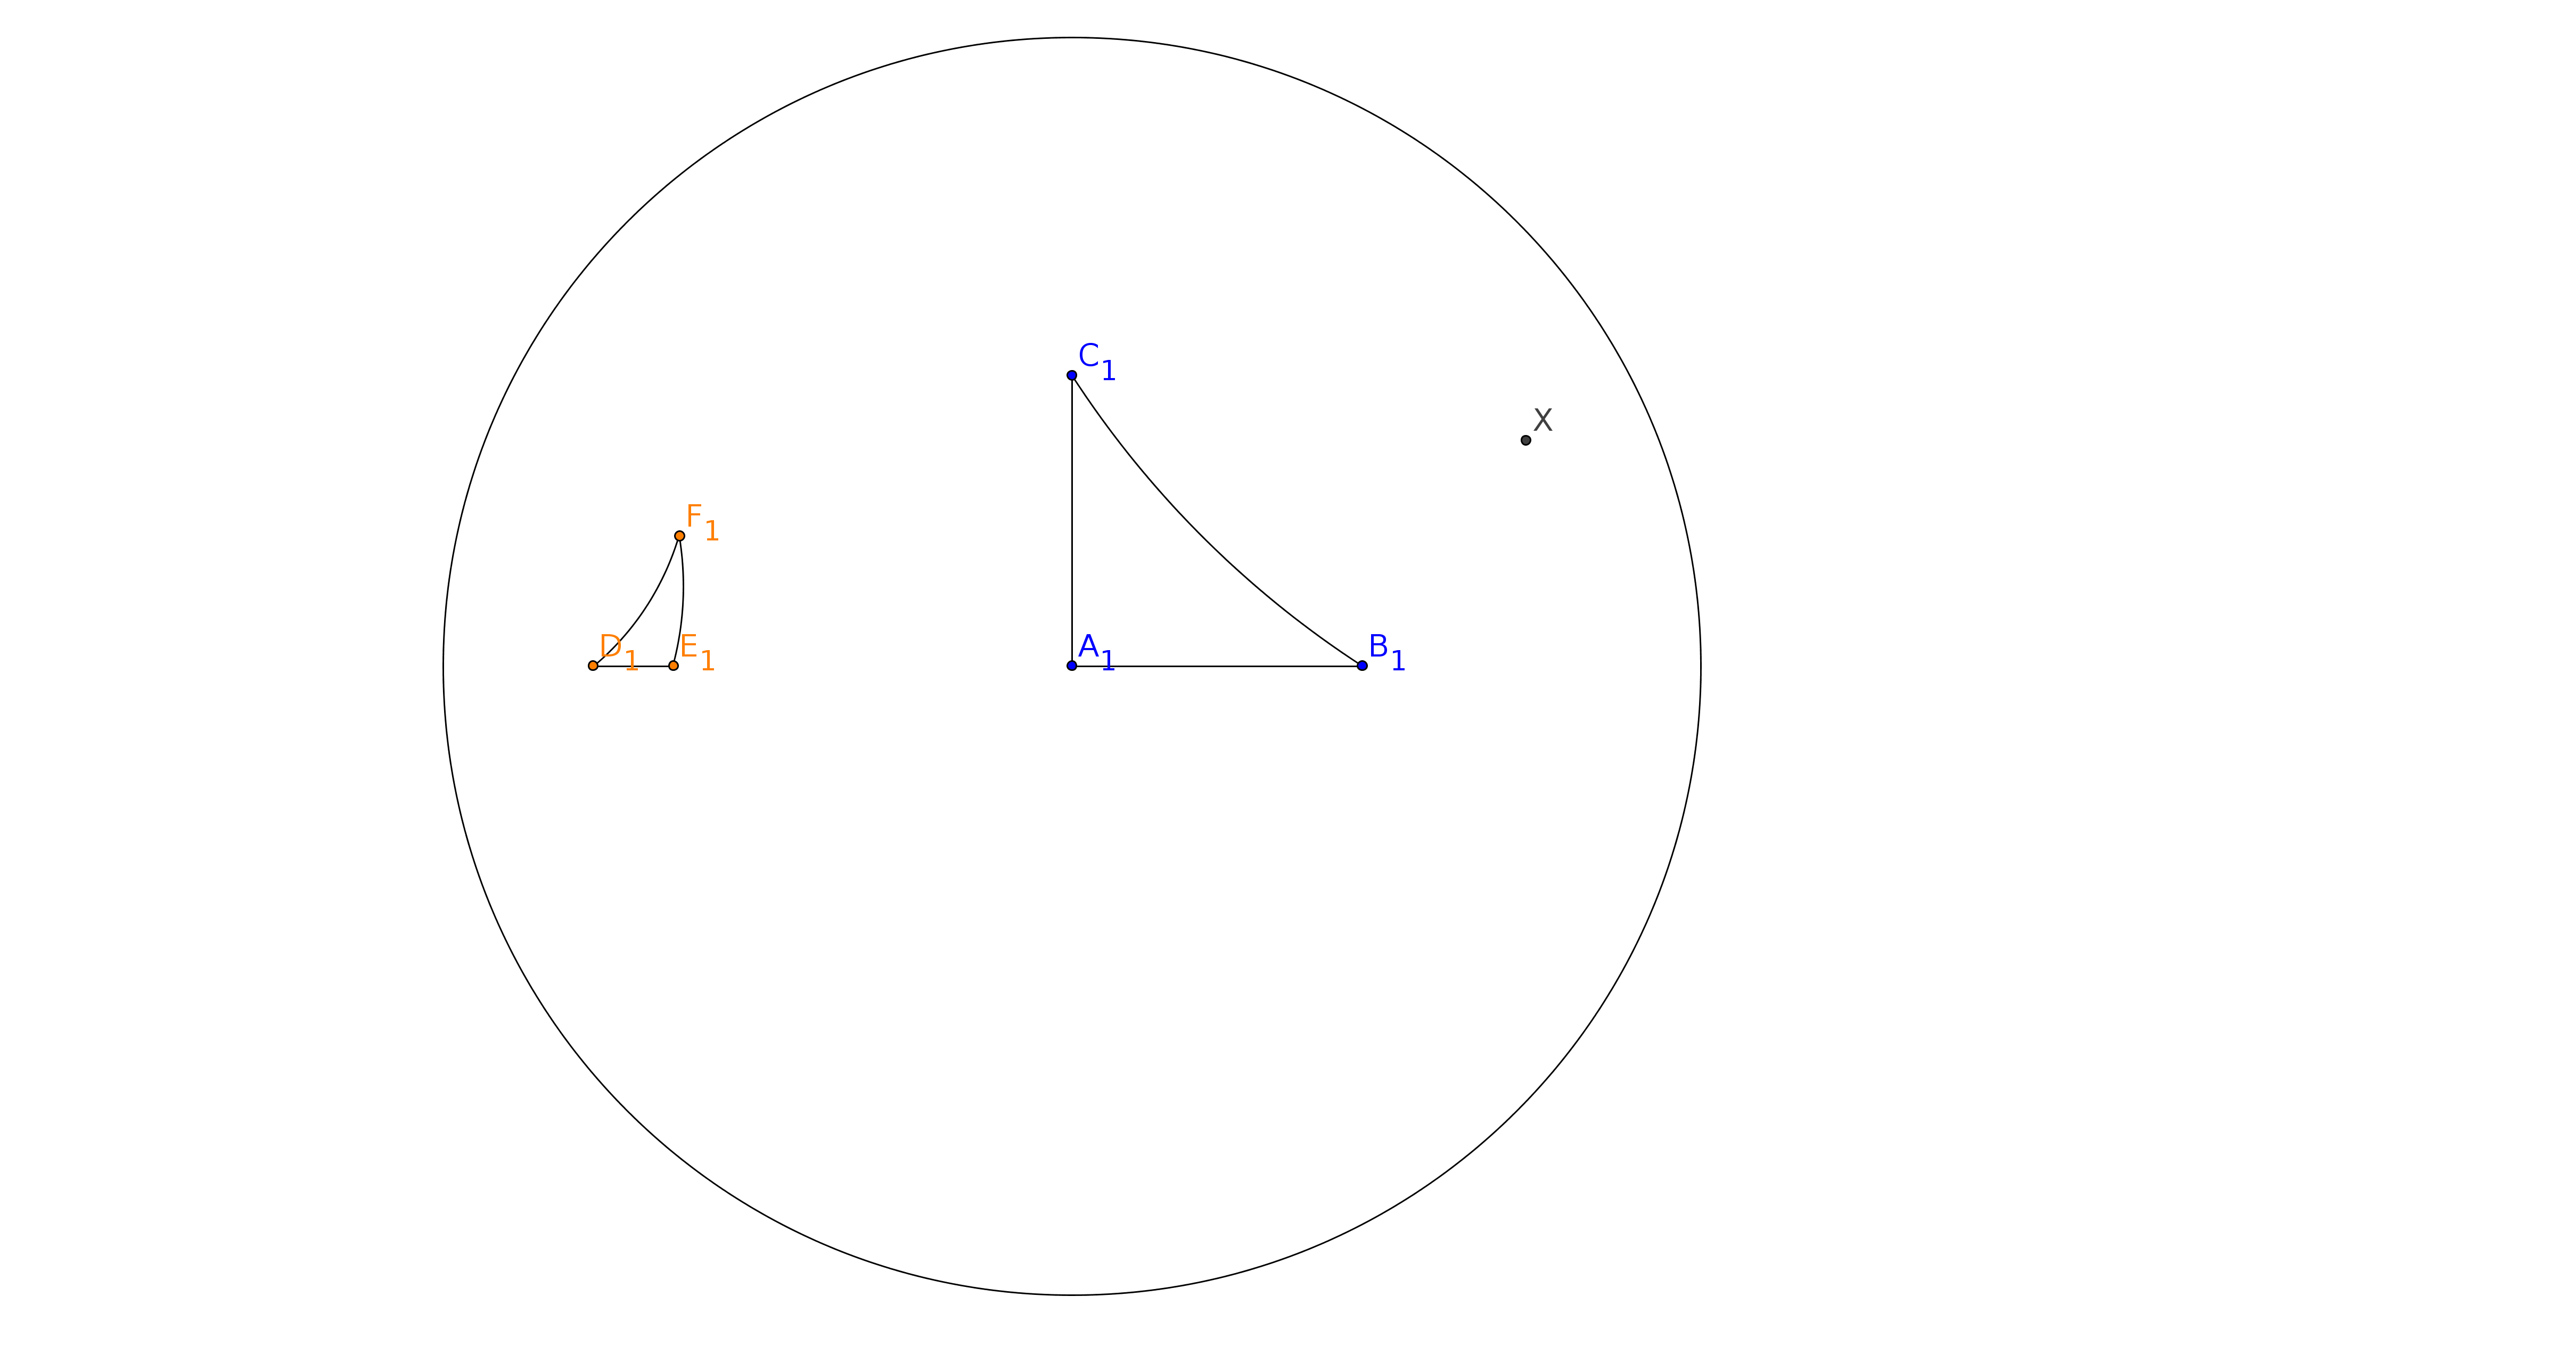
\includegraphics[width=65mm]{../images/t1_over_x.png} & 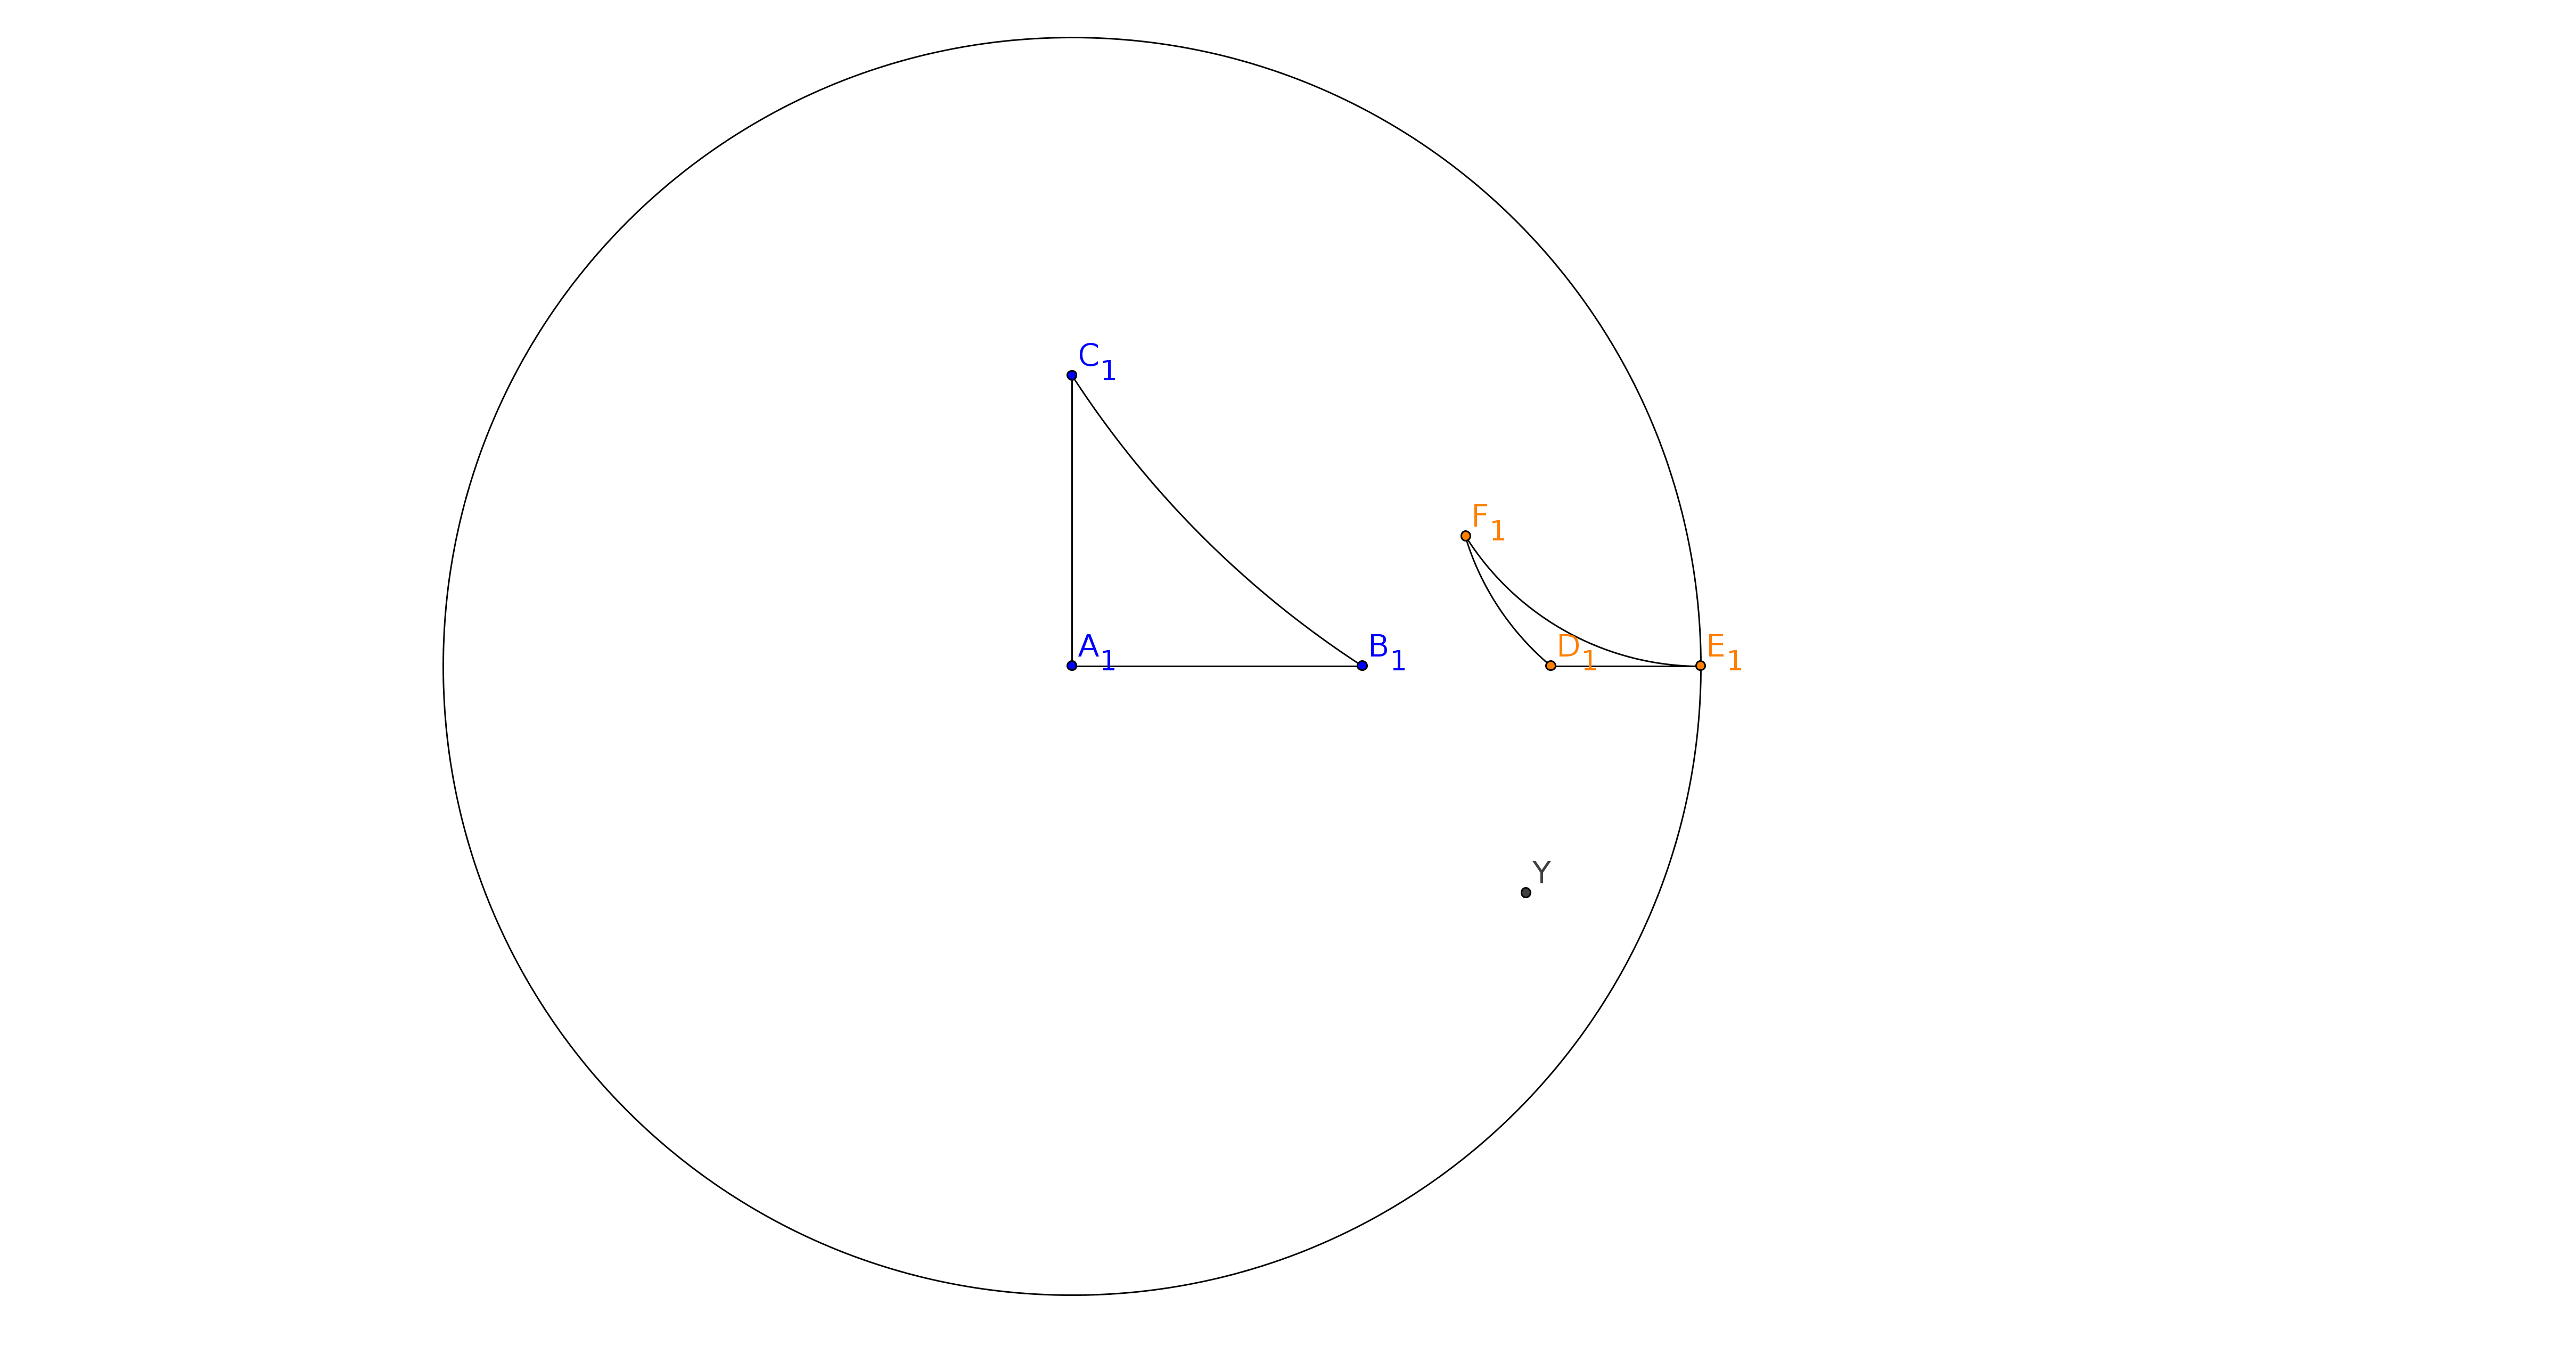
\includegraphics[width=65mm]{../images/t1_over_y.png} \\
Triangle $T_1$ over point $X$ & Triangle $T_1$ over point $Y$  \\
& \\
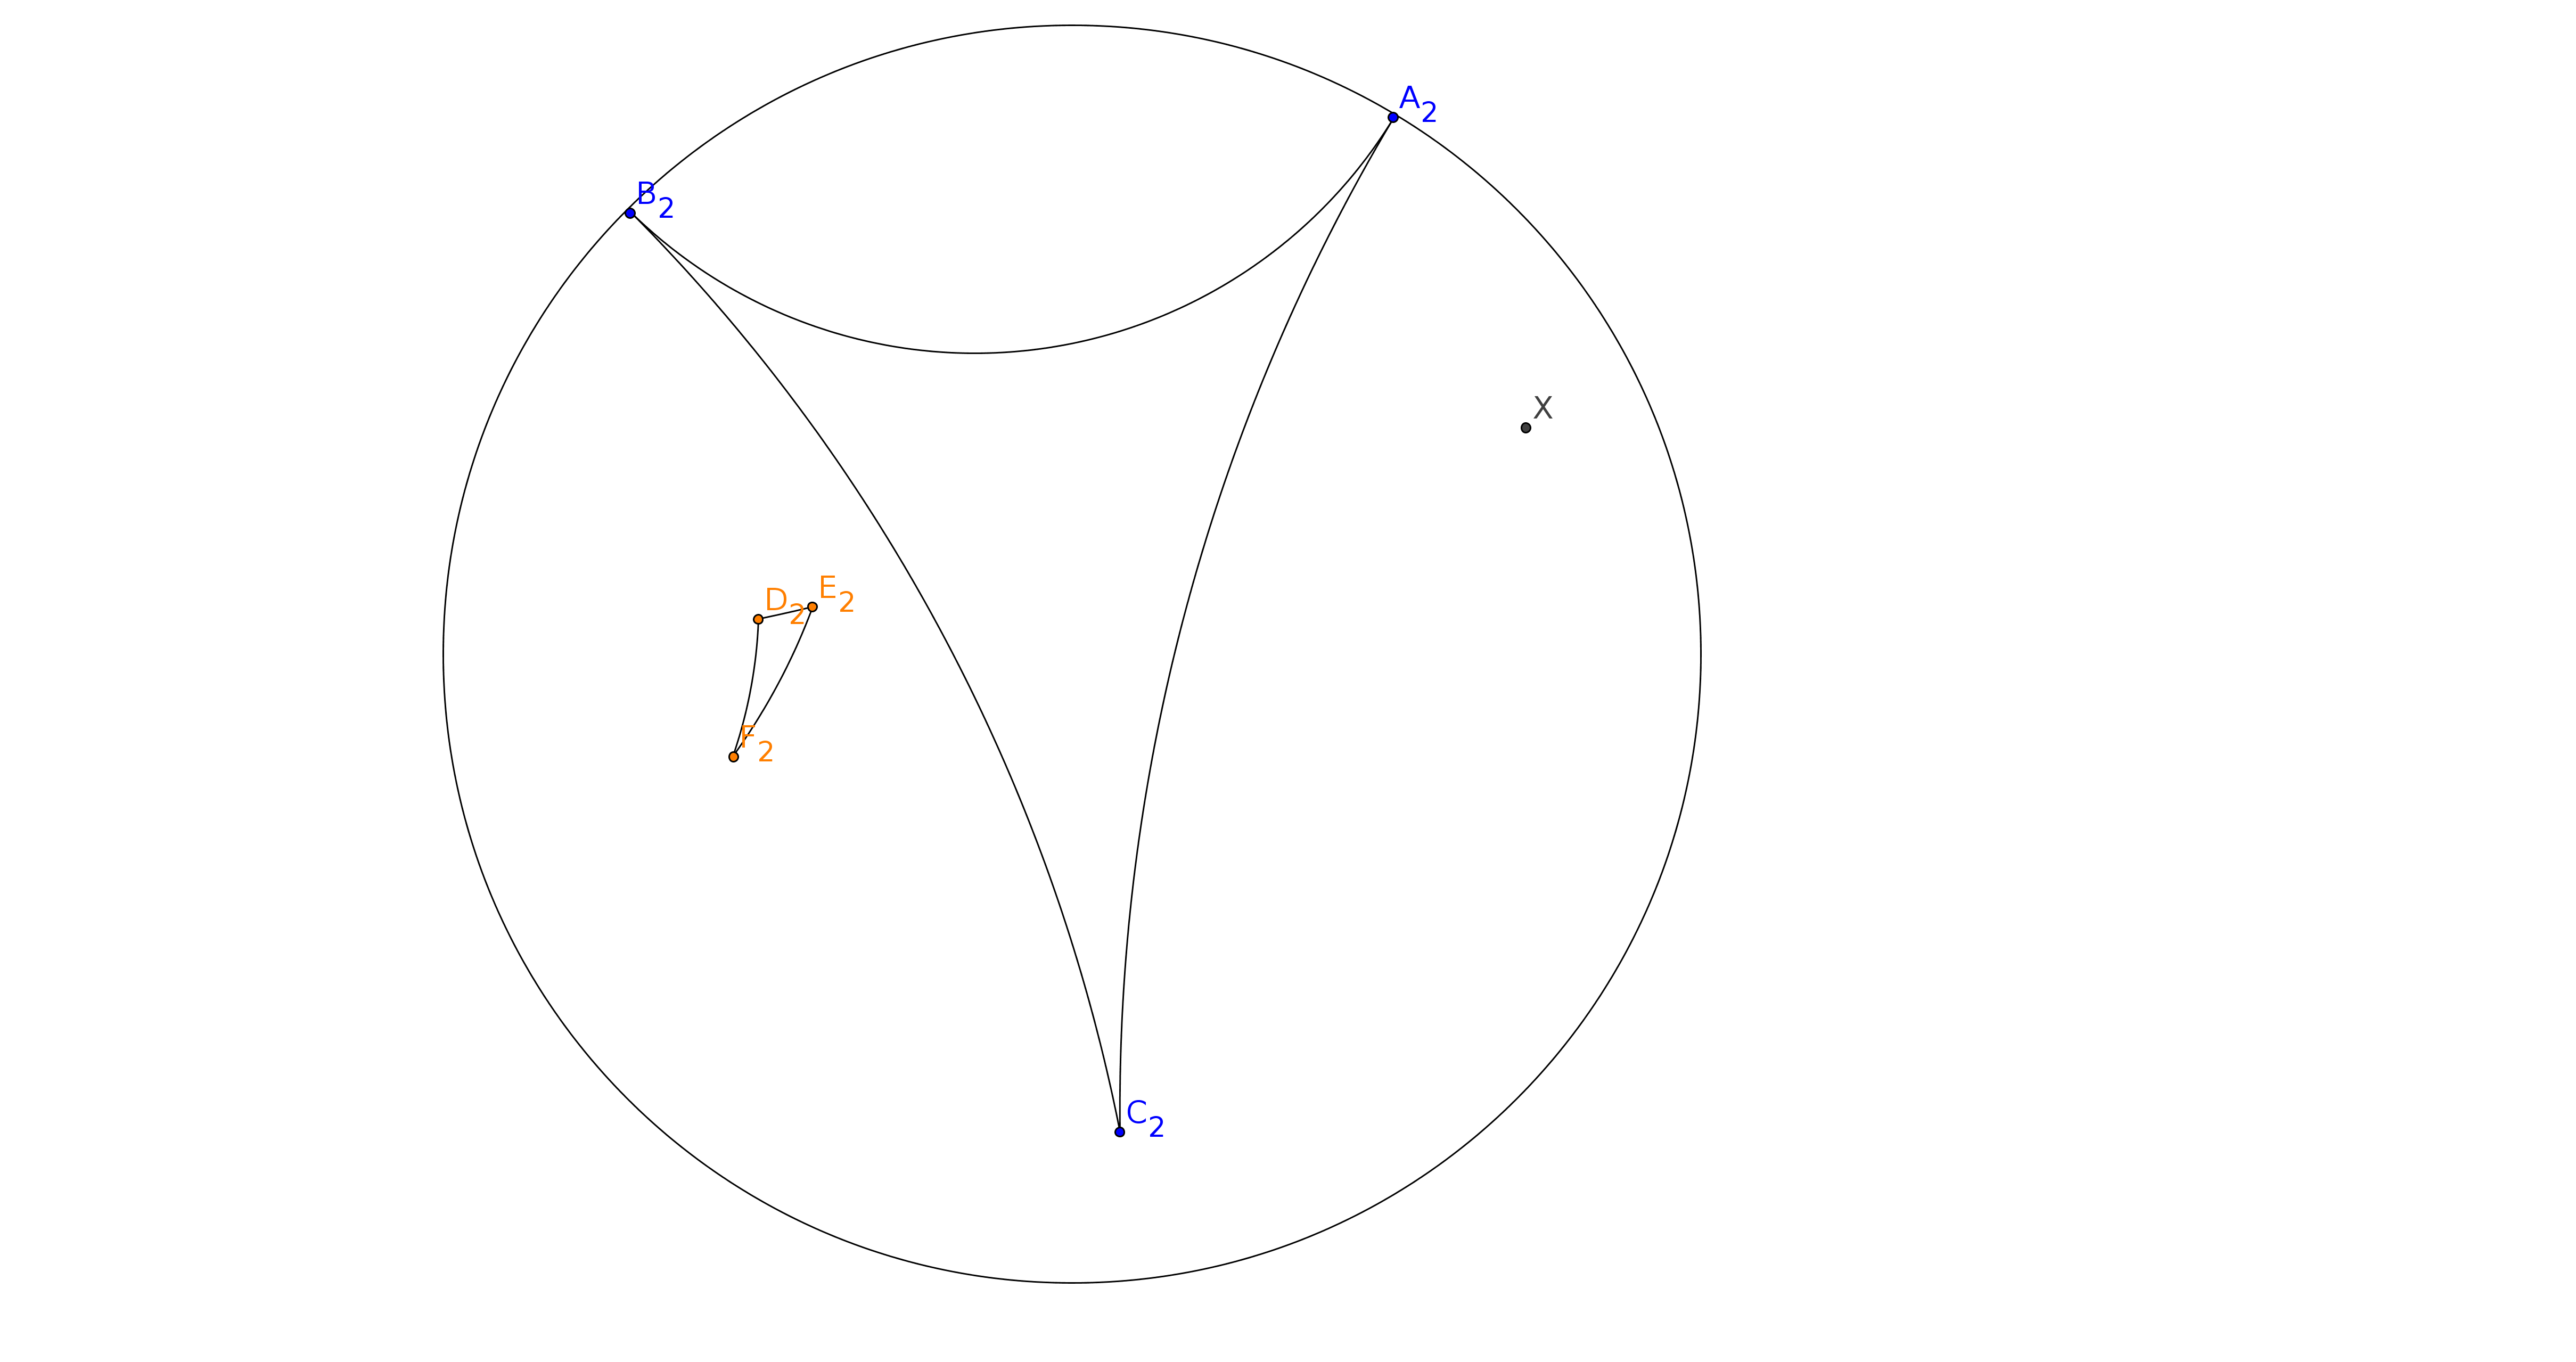
\includegraphics[width=65mm]{../images/t2_over_x.png} & 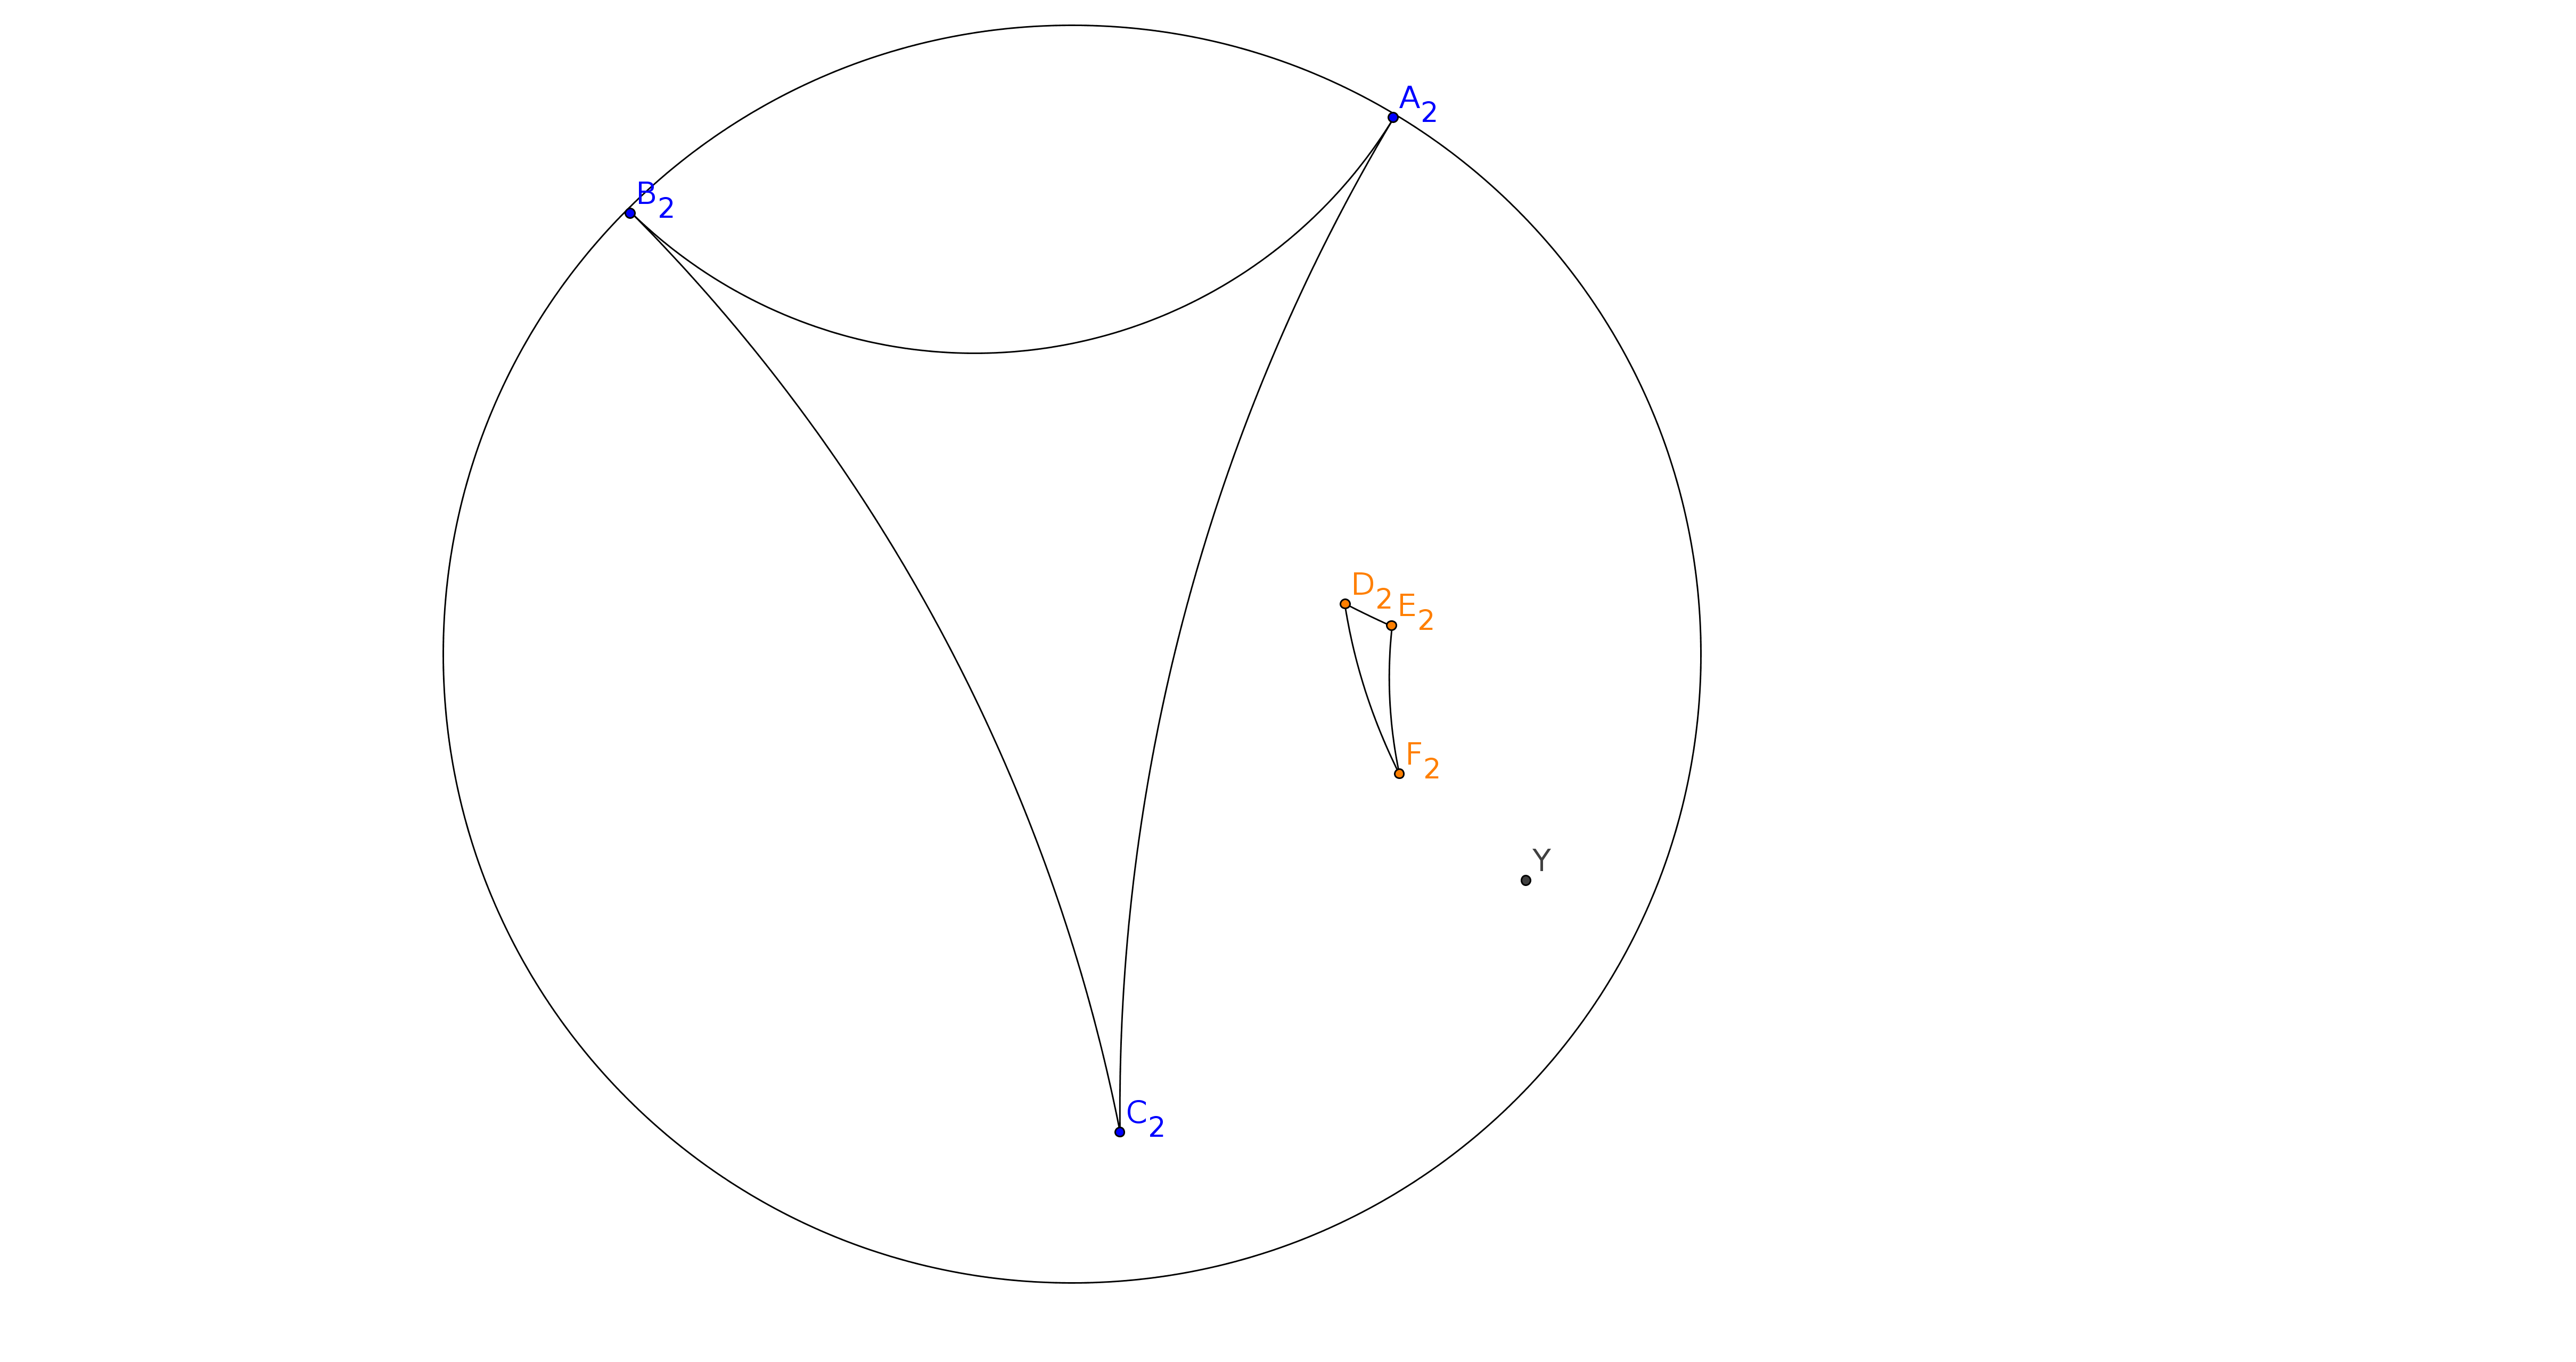
\includegraphics[width=65mm]{../images/t2_over_y.png}\\
Triangle $T_2$ over point $X$ & Triangle $T_2$ over point $Y$  \\
\end{tabular}

From these diagrams we notice two oddities. For one, these point reflections look more like line reflections than they do point reflections. That is, the triangles seem to be ``reflected" and ``stretched" rather than simply ``rotated." Also, it is unclear from these diagrams why we restricted our choice of points to those from the convex domain defined by the parabola $x = y^2$. We now discuss these issues and their implications in turn.
fx
As mentioned, these point reflections match an intuitive conception of a line reflection more than they do a point reflection. A closer look at the matrix encodings of point reflections and line reflections sheds light on this. 

\begin{theorem}
By Guggenheimer's definitions, all line reflections can be encoded as point reflections. 
\end{theorem}

\begin{proof}
Suppose that we have a line reflection $f_l$ given by $l = (l_1, l_2)$. We then encode the corresponding reflection in the matrix 
\[ M_l := \stanlinenoendmat. \]
To show that $f_l$ can be encoded as a point reflection, notice that 
\[ -1 \cdot \stanlinenoendmat = \lftmat{l_2}{l_1}{-1}{-l_2}.\]
Notice further that this matrix takes the form of a point reflection about $l = (l_1, l_2)$ if we set $\lambda = -1$. It follows that all line reflections can indeed be encoded as point reflections.
\end{proof}

Therefore the ``distinction" between line reflections and point reflections as put forth by Guggenheimer is indeed as arbitrary as it originally seemed. 

A further issue with this distinction arises once we complexify $\R$ as suggested by Guggenheimer. Because $\R^{\C} = \C$ is not ordered, there is no way to compare the determinant of a matrix $M$ with entries in $\C$ to 0. This issue will occur in all complexified fields, as no complexified field can be ordered. Thus, Guggenheimer's distinction between line reflections and point reflections by the determinant of their corresponding matrices is arbitrary and best and entirely non-applicable at worst.

Another crucial element of Guggenheimer's geometry is rendered nonsensical once we begin to work with complexified fields. In particular, his insistence that points be taken from the convex domain defined by the parabola $x = y^2$ (hereafter referred to as $D$) has no meaning in fields that are not ordered.

However, there is no clear geometric motivation behind this choice anyway. To investigate this, we reflect triangles $T_1$ and $T_2$ as defined above over a new point $Z = (-2, 1)$, which does not satisfy the condition $x > y^2$. 

\begin{tabular}{cc}
 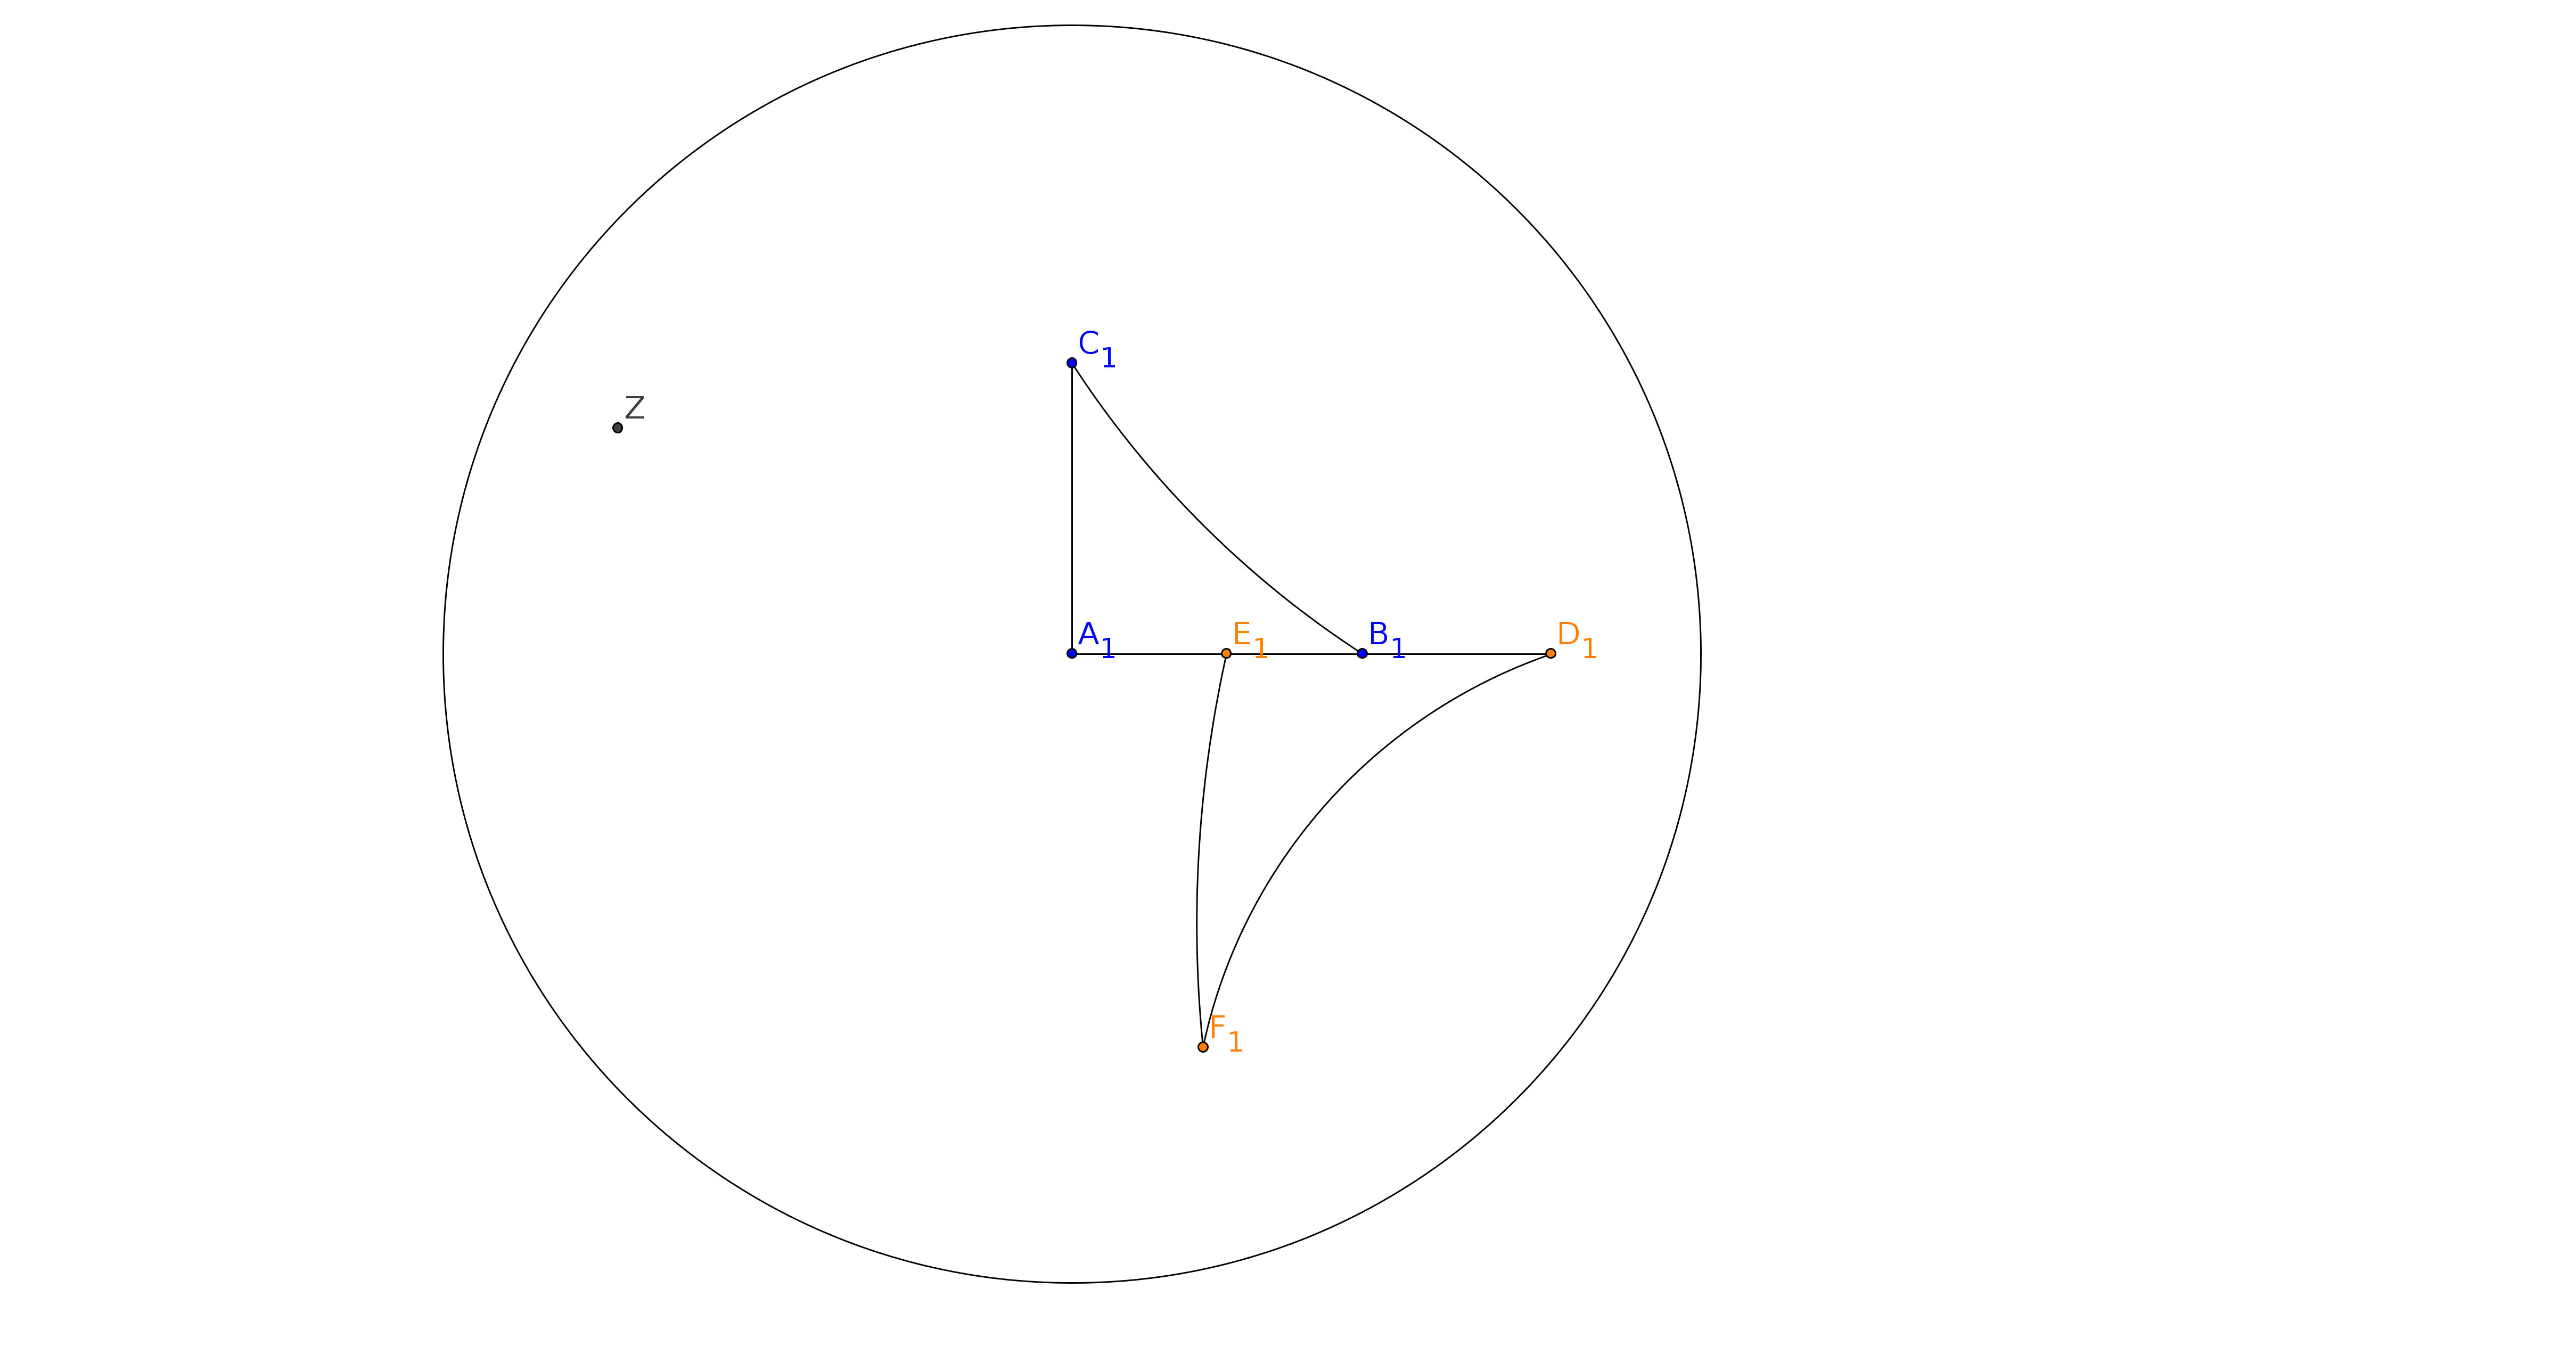
\includegraphics[width=65mm]{../images/t1_over_z.png} & 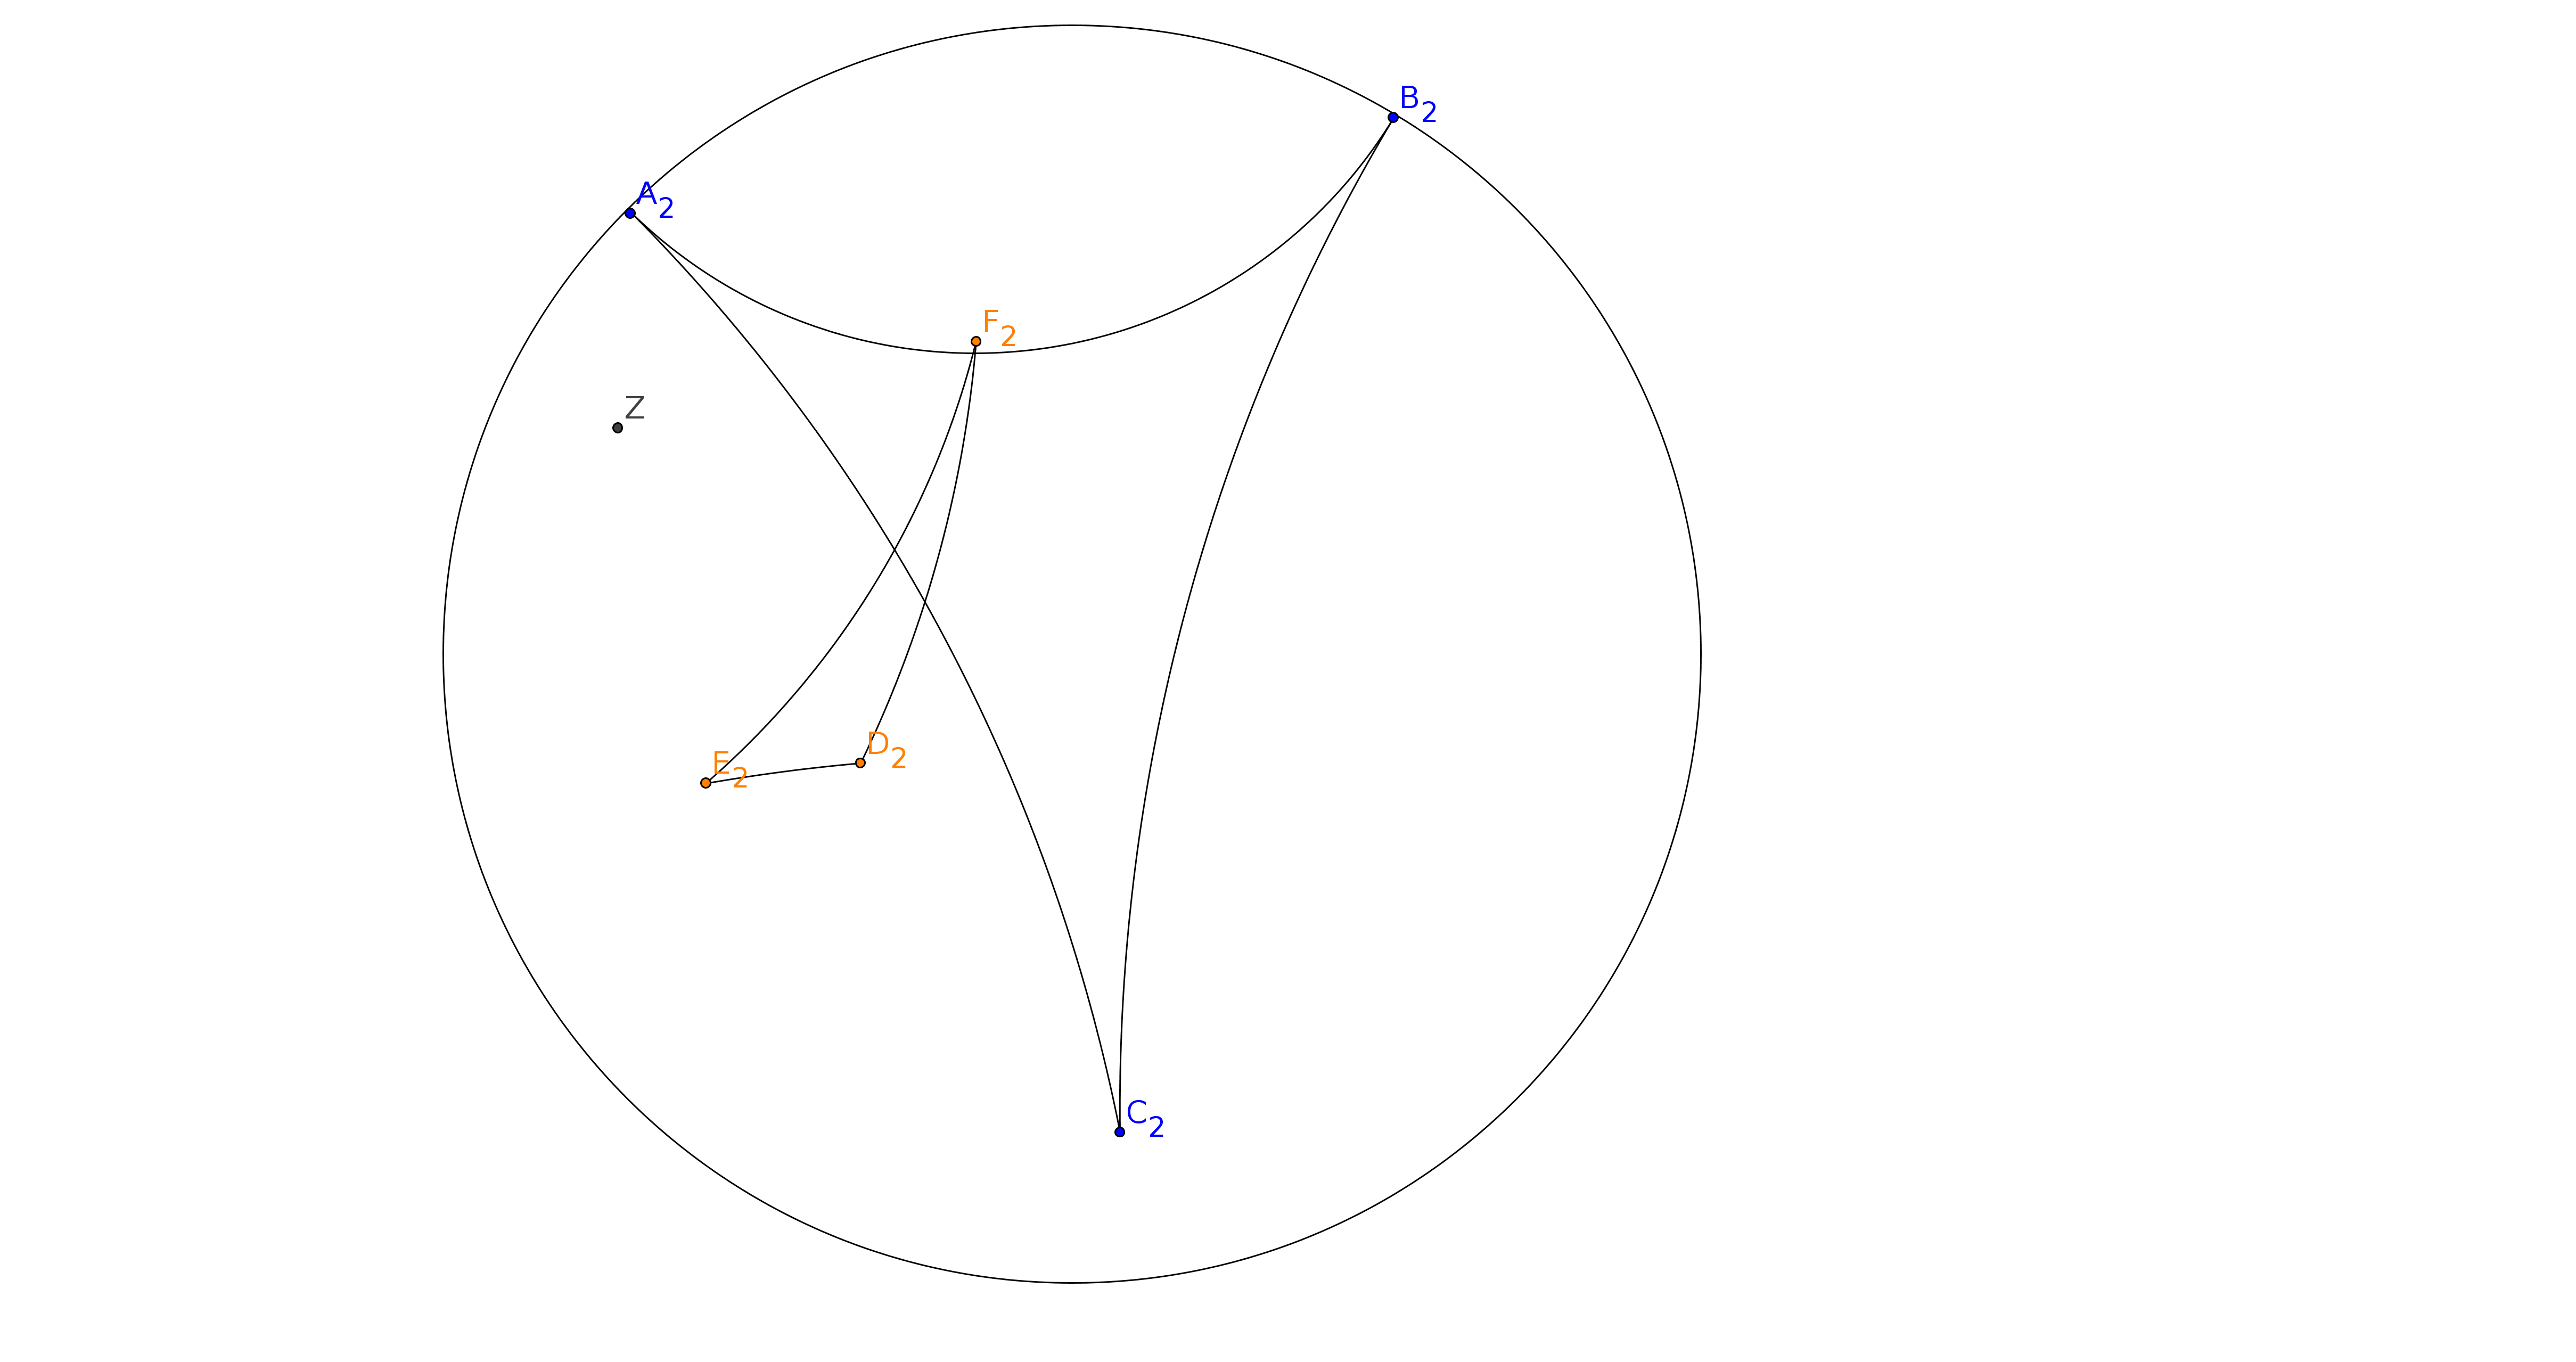
\includegraphics[width=65mm]{../images/t2_over_z.png} \\
Triangle $T_1$ over point $Z$ & Triangle $T_2$ over point $Z$  \\
& \\
\end{tabular}

Although Guggenheimer would claim that it is invalid to reflect points over $Z$ since $Z \notin D$, these reflections function similarly to those given by points within $D$. Thus, his restriction that points defining reflections must be contained in $D$ is entirely unnecessary. 

In summary, we find three problems with Guggenheimer's geometry. For one, his algebraic distinction between line reflections and point reflections appears to be largely unimportant from a geometric perspective. Similarly, his imposition of the domain $D$ has neither algebraic motivation nor geometric justification. Finally, these two crucial elements to Guggenheimer's geometry are not even applicable to fields that are unordered. It is therefore impossible to substantiate his claim that this geometry can be developed in complexified fields.



%%%%%%%%%%%%%%%%%%%%%%%%%%%%%%%%%%%%%%%%%%%%%%%%%%%%%%%%
\newpage
\begin{appendices}
\section{From $\R^2$ to the \poincare Disk} \label{appendixA}

Let $\Gamma$ be the \poincare disk. Suppose that we wish to translate the Euclidean point $A$, pictured arbitrarily below, to its equivalent point $A'$ in the \poincare disk.

\begin{center}
\begin{tikzpicture}[scale=.7]
\draw (0,0) circle (2.2cm) node[above left=1.5cm] {$\Gamma$};
\draw[fill=black] (2.2,2.2) circle (0.05) node[right] {$A$};
\end{tikzpicture}
\end{center}

We begin by constructing a line segment between $A$ and the origin $O$ and in order to find the Euclidean distance, $d_E$, between points $A$ and $O$.

\begin{center}
\begin{tikzpicture}[scale=.7]
\draw (0,0) circle (2.2cm) node[above left=1.5cm] {$\Gamma$};
\draw (0,0) -- (2.2,2.2);
\draw[fill=black] (0,0) circle (0.05) node[left] {$O$};
\draw[fill=black] (2.2,2.2) circle (0.05) node[right] {$A$};
\draw[decoration={brace,raise=4pt},decorate]
  (0,0) -- node[above left= 6pt] {$d_E$} (2.2,2.2);
\end{tikzpicture}
\end{center}

To construct the point $A'$, we want to find the radius $r$ in Euclidean distance of the circle whose hyperbolic distance from $O$ is $d_E$; $A'$ lies on this circle of radius $r$. In other words, if $d_H$ is the hyperbolic metric and $d_H(O,A') = d_E(O,A)$, then we want to find the circle, with radius $r\in\R$ centered at $O$, that contains $A'$. From \href{}{[source]} Theorem 9.1, we obtain the hyperbolic metric
\[
	d_H(O,A') = \ln\frac{1 + r}{1 - r}
\]
where $r\in\R$ is the radius of the circle we wish to draw. Let's call this new circle $\Delta$. Computing $r$, we find that
\[
	r = \frac{e^{d_H(O,A')} - 1}{e^{d_H(O,A')} + 1} =  \frac{e^{d_E(O,A)} - 1}{e^{d_E(O,A)} + 1}.
\]


Since $d_E(O,A)\in\R$, we conclude that $e^{d_E(O,A)} + 1 \neq 0$. Having computed $r$, we now draw the circle $\Delta$. 

\begin{center}
\begin{tikzpicture}[scale=.7]
\draw (0,0) circle (2.2cm) node[above left=1.5cm] {$\Gamma$};
\draw (0,0) circle (1.41cm) node[below right=.85cm] {$\Delta$};
\draw (0,0) -- (2.2,2.2);
\draw[fill=black] (0,0) circle (0.05) node[left] {$O$};
\draw[fill=black] (2.2,2.2) circle (0.05) node[right] {$A$};
\draw[fill=black] (1,1) circle (0.05) node[right] {$A'$};
\draw[decoration={brace,raise=4pt},decorate]
  (0,0) -- node[above left= 6pt] {$d_E$} (2.2,2.2);
\draw[decoration={brace,mirror,raise=4pt},decorate]
  (0,0) -- node[below right = 4pt] {$r$} (.95,.95);
\end{tikzpicture}
\end{center}

This point $A'$, the intersection between the line segment $\overline{OA}$ and $\Delta$, is the \poincare Disk-equivalent of our original point $A$.



%%%%%%%%%%%%%%%%%%%%%%%%%%%%%%%%%%%%%%%%%%%%%%%%%%%%%%%%
\newpage 
\section{The Closure of Fields under Complexification} \label{appendixB}

	Suppose $F$ is a field for which $-1$ is not the square of any number. The complexification of a field $F$ is the process of extending $F$ to a larger set by adding in the an element $i$ such that $i^2 = -1$ and then closing off under addition and multiplication. The resulting field, which we denote $F^\C$ is called the complexification of $F$ or the complexified field $F^\C$. One of the core example of complexification is the complexified reals $\R^\C$. As it turns out, this $\R^\C$ is the complex numbers $\C$. This can also be done to finite fields such as $\Z/3\Z$.

\begin{theorem} 
$\fc$ (as described above) is a field.
\end{theorem}

\begin{proof} Formally, recall that in order for $(F,+,\cdot)$ to be a field, it must satisfy the following axioms:

\begin{enumerate}
	\item $+$ must be associative and commutative.
	\item There exists an additive identity in $F$.
	\item Each $a\in F$ has an additive inverse.
	\item $\cdot$ must be associative and commutative.
	\item $+$ and $\cdot$ satisfy the distributive properties.
	\item There exists an multiplicative identity in $F$.
	\item Each $a\in F$ has an multiplicative inverse.
\end{enumerate}
Previously, all of the algebraic manipulations were carried out over a real ordered field in which all positive numbers have square roots. However, we may also carry out similar calculations over a complexified field. Let $(F,+,\cdot)$ be a field in which $-1$, the additive inverse of $1$, is not the square of any number in $F$. We define $F^\C = F\times F$. Further we define two new binary operations $\oplus$ and $\odot$ such that for all $(a,b)\ttc (c,d)\in F^\C$,
	\[
		(a,b)\oplus(c,d) = (a + c\ttc b + d)
	\]
and
	\[
		(a,b)\odot(c,d) = (ac - bd\ttc ad + bc).
	\]
wherein $+,-,\cdot$ are from $F$. We call $(F^\C,\oplus,\odot)$ the complexification of $F$. From hereon the rest of this section will be dedicated to proving the following theorem.

\begin{theorem}
	Let $(F,+,\cdot)$ be a field in which $-1$ is not a square. Then the complexification $(F^\C,\oplus,\odot)$ as defined above is a field.
\end{theorem}

\noindent First, let's resolve some properties of $\oplus$.\\

\begin{lemma}
	Given a complexification $(F^\C,\oplus,\odot)$, $\oplus$ is associative and commutative.
\end{lemma}

\begin{proof}

First we will show that $\oplus$ is associative. Let $(a,b)\ttc(c,d)\ttc(e,f)\in F^\C$.
\begin{align*}
	((a,b)\oplus(c,d))\oplus(e,f) & = (a + c\ttc b + d) + (e,f)\\
	& = ((a + c) + e\ttc (b + d) + f)\\
	& = (a + (c + e)\ttc b + (d + f)) & \text{(associativity of $+$)}\\
	& = (a,b) \oplus (c + e\ttc d + f)\\
	& = (a,b)\oplus ((c,d) \oplus (e,f))
\end{align*}
Hence $\oplus$ is associative. Now we argue that $\oplus$ is commutative. Let $(a,b)\ttc(c,d)\in F^\C$.
\begin{align*}
	(a,b)\oplus (c,d) & = (a + c\ttc b + d)\\
	& = (c + a\ttc d + b) & \text{(commutativity of $\oplus$)}\\
	& = (c,d)\oplus (a,b)
\end{align*}
Hence $\oplus$ is commutative. 
\end{proof}

Next, we argue that $F^\C$ has an additive identity.\\

\begin{lemma}
	The element $(0,0)\in F^\C$ is an additive identity.
\end{lemma}

\begin{proof}
Let $(a,b)\in F$ be arbitrary. We claim that $(0,0)\in F^\C$ is the additive identity of $F$. Using the fact that $0\in F$ is the additive identity, we obtain
	\[
		(a,b)\oplus (0,0) = (a + 0\ttc b + 0) = (a,b) = (0 + a\ttc, 0 + b) = (0,0) \oplus (a,b).
	\]
Therefore $(0,0)\in F^\C$ is an additive identity.
\end{proof} 

Since $F^\C$ has an additive identity, we may conjecture that $F^\C$ has additive inverses. 

\begin{lemma}
	For all $(x,y)\in F^\C$, there exists $(a,b)\in F^\C$ with 
	\[	
		(x,y)\oplus (a,b) = (0,0) = (a,b)\oplus (x,y).
	\]
	In other words, $F^\C$ has additive inverses.
\end{lemma}

\begin{proof}
Let $(a,b)\in F^\C$ be arbitrary. We claim that $(-a,-b)\in F^\C$ is the additive inverse of $(a,b)$. Note that since $F$ is a field, $-a\ttc -b$ exist and so $(-a,-b)\in F^\C$. Furthermore,
	\[
		(a,b)\oplus (-a,-b) = (a + -a\ttc b + -b) = (0,0) = (-a + a\ttc, -b + b) = (-a,-b) \oplus (a,b).
	\]
	Hence $\oplus$ is closed under inverses.
\end{proof}

Now we've proved that $\oplus$ has the desired properties that addition needs in a field. We therefore set our sights on resolving the properties of $\odot$.\\

\begin{lemma}
	The operation $\odot$ is associative and commutative.
\end{lemma}

\begin{proof}
	Now we argue via a similar line of reasoning that $\odot$ satisfies the properties of field multiplication. First we claim that $\odot$ is associative. Let $(a,b)\ttc(c,d)\ttc(e,f)\in F^\C$ be arbitrary. Using distributivity in $F$ and associativity and commutativity of $+$ and $\cdot$, we obtain
\begin{align*}
		((a,b)\odot(c,d))\odot(e,f) & = (ac - bd\ttc ad + bc)\odot (e,f)\\
		& = ((ac - bd)e - (ad + bc)f\ttc (ac - bd)f + (ad + bc)e)\\
		& = (ace - bde - adf - bcf\ttc acf - bdf + ade + bce)\\
		& = (a(ce - df) - b(de + cf)\ttc b(ce - df) + a(de + cf))\\
		& = (a,b)\odot (ce - df\ttc de + cf)\\
		& = (a,b)\odot ((c,d)\odot (e,f))
\end{align*}
Hence $\odot$ is associative. Now we show that $\odot$ is commutative. Let $(a,b)\ttc(c,d)\in F^\C$ be arbitrary. Then
	\begin{align*}
		(a,b)\odot (c,d) & = (ac - bd\ttc ad + bc)\\
		& = (ca - db\ttc da + cb) & \text{(commutativity of $\cdot$)}\\
		& = (c,d)\odot (a,b)
	\end{align*}
	Therefore $\odot$ is commutative.
\end{proof}

With these properties in mind, we now show that $F^\C$'s operations obey the distributive property.\\

\begin{lemma}
	The complexification $(F^\C,\oplus,\odot)$ obeys the distributive property.
\end{lemma}

\begin{proof}
Next we show that $F^\C$ has the distributive property. Let $(a,b)\ttc(c,d)\ttc(e,f)\in F^\C$ be arbitrary. Since $\odot$ is commutative, it suffices to argue that
	\[
		(a,b)\odot((c,d)\oplus(e,f)) = (a,b)\odot(c,d)\oplus(a,b)\odot(e,f).
	\]
	Following previous arguments, we find that
	\begin{align*}
		(a,b)\odot((c,d)\oplus(e,f)) & = (a,b)\odot(c + e\ttc d + f)\\
		& = (a(c + e) - b(d + f)\ttc a(d + f) + b(c + e))\\
		& = (ac + ae - bd - bf\ttc ad + af + bc + be) & \intertext{(distributivity in $F^\C$)}
		& = ((ac - bd) + (ae - bf)\ttc (ad + bc) + (af + be)) & \intertext{(commutativity and associativity of $+$)}
		& = (ac - bd\ttc ad + bc)\oplus (ae - bf\ttc af + be)\\
		& = (a,b)\odot (c,d)\oplus (a,b)\odot(e,f)
	\end{align*}
	Hence $F^\C$ has the distributive property. 
\end{proof}	

Since $F^\C$ satisfies the distributive property, we only have two properties left to demonstrate: multiplicative identities and multiplicative inverses. \\

\begin{lemma}
	The element $(1,0)\in F^\C$ is a multiplicative identity.
\end{lemma}

\begin{proof}
We claim that $(1,0)$ is the multiplicative identity of $F^\C$. Let $(a,b)\in F^\C$ be arbitrary. Note that since $F$ is a field, $1\in F$ is the multiplicative identity. Then
	\[
		(a,b)\odot(1,0) = (a\cdot 1 - b\cdot 0\ttc a\cdot 0 + b\cdot 1) = (a,b) = (1\cdot a - 0\cdot b\ttc 0\cdot a + 1\cdot b) = (1,0)\cdot (a,b).
	\]
	Hence $F^\C$ has a multiplicative identity.
\end{proof}

Since $F^\C$ has a multiplicative identity, we may conjecture that $F^\C$ has multiplicative inverses. \\
 
\begin{lemma}
	For all $(x,y)\in F^\C\backslash\{(0,0)\}$, there exists $(a,b)\in F^\C\backslash\{(0,0)\}$ with 
	\[	
		(x,y)\odot (a,b) = (1,0) = (a,b)\odot (x,y).
	\]
	In other words, $F^\C$ has multiplicative inverses.	
\end{lemma} 

\begin{proof}
Suppose $(a,b)\in F^\C\backslash\{(0,0)\}$. We hope to find $(x,y)\in F^\C$ with the property $(a,b)\odot(x,y) = (1,0)$. Since $\odot$ is commutative, this result holds for $(x,y)\odot(a,b)$ as well. Performing the multiplication, we find that
	\[
		(a,b)\odot(x,y) = (ax - by\ttc ay + bx) = (1,0)
	\]
	and so we obtain the equations
	\begin{align*}
		ax - by & = 1\\
		ay + bx & = 0
	\end{align*}
	Now we need to solve for $x$ and $y$. Multiply the upper equation by $a$ and the lower equation by $b$ to obtain
	\begin{align*}
		a^2x - aby & = a\\
		aby - b^2x & = 0
	\end{align*}
	Adding the two equations together, we find that
	\[
		x = \frac{a}{a^2 + b^2}.
	\]
	Via a similar process of multiplying the first equation by $b$ and the second equation by $a$ and adding the results, we also obtain
	\[
		y = \frac{-b}{a^2 + b^2}.
	\]
	Now we hope that there is no $(a,b)\in F^\C\backslash\{(0,0)\}$ with $a^2 + b^2 = 0$. Suppose such values do exist however. Since $(a,b)\neq (0,0)$, suppose $a\neq 0$. Then we conclude that
	\begin{align*}
		a^2 + b^2 = 0 & \text{ which implies } b^2 = -a^2\\
		& \text{ which implies } \frac{b^2}{a^2} = -1\\
		& \text{ which implies } \left(\frac{b}{a}\right)^2 = -1.
	\end{align*}
 	In other words, $-1$ is the square of $\frac{b}{a}\in F$, a contradiction since we assumed that no element in $F$ had $-1$ as its square. A similar argument can be made for when $b \neq 0$ using the fraction $\frac{a}{b}$. Hence $a^2 + b^2 \neq 0$ for any $(a,b)\in F^\C\backslash\{(0,0)\}$. Therefore $F^\C$ has multiplicative inverses.
\end{proof} 	
 	
Combining these seven lemmas, we conclude that $(F^\C,\oplus,\odot)$ is a field as desired. Hence the theorem is true and so the complexification of a field is a field. 

\end{proof}



%%%%%%%%%%%%%%%%%%%%%%%%%%%%%%%%%%%%%%%%%%%%%%%%%%%%%%%%
\newpage 
\section{Encoding LFTs as Matrices} \label{appendixC}

\noindent Define the set
	\[
		A = \left\lbrace z\mapsto \frac{az + b}{cz + d}\colon a,b,c,d\in F\text{ with } ad - bc \neq 0\right\rbrace
	\]
of linear fractional transformations under function composition and let $GL_2(F)$ denote the group of invertible $2\times 2$ matrices with entries in $F$. Also define the subset
	\[
		F^* = \left\lbrace\lftmat{\lambda}{0}{0}{\lambda}\colon \lambda\in F\text{ with } \lambda\neq 0 \right\rbrace.
	\]
	We argue that $F^*$ is a normal subgroup of $GL_2(F)$.
\begin{lemma}
	The subset $F^*$ defined above forms a normal subgroup of $GL_2(F)$.
\end{lemma}
\begin{proof}
	Let $F^*$ be defined as above. We first argue that $F^*$ is a subgroup of $GL_2(F)$. Let $A,B\in F^*$ be arbitrary. Then
	\[
		AB = \lftmat{\lambda_A}{0}{0}{\lambda_A}\lftmat{\lambda_B}{0}{0}{\lambda_B} = \lftmat{\lambda_A\lambda_B}{0}{0}{\lambda_A\lambda_B}
	\]
	and since $\lambda_A\lambda_B\in F$ and $F$ has no zero divisors, we conclude that $AB\in F^*$. It's worth noting that the matrices in $F^*$ commute with one another since $\lambda_A\lambda_B = \lambda_B\lambda_A$. From here, notice that the identity element of $F^*$ remains the identity matrix as
	\[
		AI = \lftmat{\lambda_A}{0}{0}{\lambda_A}\lftmat{1}{0}{0}{1} = A
	\]
	and $IA = A$ by commutativity. In a similar vain, if $A\in F^*$ has entry $\lambda_A$, then $B\in F^*$ with $\lambda_B = \frac{1}{\lambda_A}$ is the inverse of $A\in F^*$, following from the assumption that $\lambda_A \neq 0$. Hence $F^*$ forms a subgroup of $GL_2(F)$. Now we show that $F^*$ is normal. Let $A\in GL_2(F)$ and choose some $B\in F^*$. We argue that $AB = CA$ for some $C\in F^*$. Observe that
	\[
		AB = \stanlftmat\lftmat{\lambda_B}{0}{0}{\lambda_B} = \lftmat{a\lambda_B}{b\lambda_B}{c\lambda_B}{d\lambda_B} = \lftmat{\lambda_B a}{\lambda_B b}{\lambda_B c}{\lambda_B d} = \lftmat{\lambda_B}{0}{0}{\lambda_B}\stanlftmat = BA.
	\]
	Therefore $F^*$ is normal as desired.
\end{proof}
	
With this in mind, we now define the map $\varphi\colon A\rightarrow GL_2(F)/F^*$ by

	\[
		\varphi\left(z\mapsto \frac{az + b}{cz + d}\right) = \stanlftmat F^*
	\]
	We claim that $\varphi$ is a surjective homomorphism.
\begin{theorem}
		The map $\varphi\colon A\rightarrow GL_2(F)/F^*$ given above is a surjective homomorphism with $\ker(\varphi)$ given by the set
		\[
			\left\lbrace z\mapsto \frac{az + b}{cz + d}\colon a = d\neq 0\text{ and } b = c = 0\right\rbrace.
		\]
\end{theorem}

Effectively, we lose injectivity because we may have linear fractional transformations that differ by the same constant multiple in the numerator and denominator. More concretely, if $\lambda \neq 0$ with $a + b = a\lambda + b\lambda$ and $c + d = c\lambda + d\lambda$, then the maps
\[
	z\mapsto\frac{az + b}{cz + d}\quad\text{ and }\quad z\mapsto\frac{a\lambda z + b\lambda}{c\lambda z + d\lambda}
\]  
are the same.
	
\begin{proof}
	First, we argue that $\varphi$ is a homomorphism. Let $f,g\in A$ be two distinct maps. Notice that
	\begin{align*}
		\varphi(g\circ f) & = \varphi\left(g\left(\frac{a_fz + b_f}{c_fz + d}\right)\right)\\
		& = \varphi\left(\frac{a_g\frac{a_fz + b_f}{c_fz + d_f} + b_g}{c_g\frac{a_fz + b_f}{c_fz + d_f} + d_g}\right)\\
		& = \varphi\left(\frac{a_ga_fz + a_gb_f + b_gc_fz + b_gd_f}{c_ga_fz + c_gb_f + d_gc_fz + d_gd_f}\right) & \text{(simplifying common denominators)}\\
		& = \varphi\left(\frac{(a_ga_f + b_gc_f)z + (a_gb_f + b_gd_f)}{(c_ga_f + d_gc_f)z + (c_gb_f + d_gd_f)}\right) & \text{(grouping terms for $\varphi$)}\\
		& = \lftmat{a_ga_f + b_gc_f}{a_gb_f + b_gd_f}{c_ga_f + d_gc_f}{c_gb_f + d_gd_f} F^*\\
		& = \lftmat{a_g}{b_g}{c_g}{d_g}\lftmat{a_f}{b_f}{c_f}{d_f}F^*\\
		& = \varphi(g)\varphi(f)F^*
	\end{align*}
	Hence $\varphi$ is a homomorphism. Now we argue that $\varphi$ is surjective. Suppose $M F^*\in GL_2(F)/F^*$ is some matrix with entries $a,b,c,d$. Then the linear fractional transformation given by 
	\[
		f(z) = \frac{az + b}{cz + d}
	\]
	is mapped to $M F^*$ by $\varphi$. Hence $\varphi$ is a surjective homomorphism. Now, notice that if a map $f$ is in $\ker(\varphi)$, then 
\end{proof}		
	

\begin{corollary}
	The groups $A/\ker(\varphi)$ and $GL_2(F)/F^*$ are isomorphic.
\end{corollary}
\begin{proof}
	Apply the First Isomorphism Theorem for groups to $A$ using the fact that $\Range(\varphi) = GL_2(F)/F^*$.
\end{proof}

\newpage
\section{Code Simulating LFTs} \label{appendixD}

Below is the code we used to apply point reflections and line reflections to various points in $\C$. 

\lstinputlisting[language=Python]{../python/code.py}

\end{appendices}



%%%%%%%%%%%%%%%%%%%%%%%%%%%%%%%%%%%%%%%%%%%%%%%%%%%%%%%%
\newpage
\section*{``Bibliography" (List of Sources)}

\begin{enumerate}
	\item H. Guggenheimer, Plane Geometry and Its Groups, Holden-Day San Francisco (now Kreiger, Huntington N.Y.), 1967, Chap, 9.
	\item Guggenheimer's paper itself
	\item Robin Hartshorne, Geometry: Euclid And Beyond, Srpinger-Verlag New York, 2000, Chap, 7.
	\item \href{http://people.reed.edu/mayer/math112.html/chap04.pdf}{http://people.reed.edu/mayer/math112.html/chap04.pdf}
	\item \href{https://www.geogebra.org/material/show/id/7005}{https://www.geogebra.org/material/show/id/7005}
	\item \href{https://www.geogebra.org/home}{https://www.geogebra.org/home}
	\item \href{https://pdfs.semanticscholar.org/ed0e/d1fee9bbe60b24be373ac1207d17ecb90b4a.pdf}{https://pdfs.semanticscholar.org/ed0e/d1fee9bbe60b24be373ac1207d17ecb90b4a.pdf}
	\item \href{http://math2.uncc.edu/~frothe/3181alllhyp1_7.pdf}{http://math2.uncc.edu/$\sim$frothe/3181alllhyp1$\_$7.pdf}
\end{enumerate}

\end{document}